%
\documentclass[11pt]{report}
\usepackage{etex}
\usepackage[letterpaper, top=1in, bottom=1.25in, left=1.25in, right=1.25in]{geometry}
\usepackage[pdftex]{graphicx}
\usepackage{amsmath,amssymb,latexsym}
\usepackage[style=numeric,sorting=nty]{biblatex}
\usepackage{tipa,textcomp,enumerate}
\usepackage{fancyhdr,tabularx,tabulary}
\usepackage{paralist,comment,fancyvrb}
\usepackage{multirow,url,calc}
\usepackage[group-separator={,}]{siunitx}
\usepackage{pgfplots,xmpincl}
\usepackage{epstopdf}
\usepackage[nottoc,numbib]{tocbibind}
\usepackage{color,colortbl}
\usepackage{draftwatermark}

\newcommand*\mean[1]{\overline{#1}}

\addbibresource{bibdata.bib}

\newcommand{\mtilde}{$\mathtt{\sim}$}
\usepackage{listings}% http://ctan.org/pkg/listings
\lstset{
  basicstyle=\ttfamily,
  mathescape
}

\SetWatermarkScale{3}

\usetikzlibrary{arrows.meta}
\usetikzlibrary{patterns}
\pgfplotsset{compat=1.12}

% use with tikz to create Normal distribution
\pgfmathdeclarefunction{gauss}{2}{%
  \pgfmathparse{1/(#2*sqrt(2*pi))*exp(-((x-#1)^2)/(2*#2^2))}%
}

\graphicspath{ {images/} }
\includexmp{metadata/CC_Attribution_4.0_International}

% to create matrices that represent games in normal form
% with better spacing for readability and with vertical lines
% that do not extend over all rows.
\newcommand{\gtcol}[1]{\multicolumn{1}{c|}{#1}}
\newcolumntype{Y}{>{\centering\arraybackslash}X}

\includecomment{solution}
%\excludecomment{solution} % comment this out to create the solutions
\newcommand{\bs}{\textbf{Solution.}~}

\setcounter{secnumdepth}{2}
\setcounter{tocdepth}{1}

\begin{document}
\chapter*{\Huge \center An Introduction to Prescriptive
  and Predictive Modeling}
\thispagestyle{empty}
%{\hspace{0.25in} \includegraphics{./ru_sun.jpg} }
%\section*{\large \center Darin England}

\newpage
\noindent
An Introduction to Prescriptive and Predictive Modeling\\
Copyright \copyright 2020 by Darin England\\
\includegraphics[scale=0.8]{by-nc.eps}\\
This work is licensed under the Creative Commons Attribution-NonCommercial 4.0
International License. To view a copy of this license,
visit \url{http://creativecommons.org/licenses/by-nc/4.0/}.
You are free to:\\
Share – copy and redistribute the material in any medium or format\\
Adapt – remix, transform, and build upon the material\\
The licensor cannot revoke these freedoms as long as you follow the license terms.
Under the following terms:\\
Attribution – You must give appropriate credit, provide a link to the license,
and indicate if changes were made. You may do so in any reasonable manner,
but not in any way that suggests the licensor endorses you or your use.\\
NonCommercial – You may not use the material for commercial purposes.\\
Although every precaution has been taken to verify the accuracy of the
information contained herein, the author and publisher assume no
responsibility for any errors or omissions. No liability is assumed
for damages that may result from the use of information contained
within.

\tableofcontents

\chapter{Prescriptive Modeling}

\section{Linear Programming}

The best way to learn the art of mathematical modeling is through practice.
We begin with a simple two-variable Linear Programming model whose solution
will inform the owner of a business how to allocate scarce resources to achieve
maximum profit. Additional information returned with the solution will be used
to gain insight on obtaining additional resources and an idea of the robustness
of the solution to small changes in the data.
Along the way we will
illustrate various features of the GAMS algebraic modeling language. 
\footnote{We do not provide a complete introduction to GAMS.
Excellent tutorials already exist. \cite{Rosenthal,GAMS}.}

Why use GAMS? Well, it's not GAMS in particular, but rather
algebraic modeling languages in general that are extremely useful
when \emph{formulating} mathematical programming problems
\footnote{AMPL is another popular algebraic modeling language with a 
clear and expressive syntax \cite{fourer:2003}.} An
algebraic modeling language allows one to easily specify and
understand objective functions, constraints, and logical relationships
among variables. The syntax of the GAMS language is simple,
yet expressive enough to enable many different types of problems to be
directly modeled. We should note that GAMS is not a general-purpose
programming language, although it does contain constructs for
conditional execution of statements and for iterative looping.
Rather, GAMS is an example of a \emph{domain-specific} language.  Its
purpose is to facilitate translation from a problem description into a
form that is suitable for a solver to process.

\emph{A resource allocation problem.}
A local farmer maintains 500 acres on which she can grow feed corn for animals
and/or organic corn for local millers. As the planting season approaches,
she must decide how many acres to allocate to each type of corn.
Her operating budget is \$\num{50000}. The costs and returns for each
type of corn are as follows.

\vspace{.1in}
\begin{tabular}{rrr}
type & cost per acre & revenue per acre \\ \hline
feed corn & \$90 & \$200 \\
organic corn & \$150 & \$300
\end{tabular}
\vspace{.1in}

A natural objective is to maximize total profit, and organic appears to be 
more attractive; however, the farmer must
respect both her operating budget and the available acres. If we let $x1$ and 
$x_2$ represent the 
number of acres to allocate to feed corn and organic corn, respectively,
then the farmer's decision problem is to
\[
\begin{array}{lrrrrrl}
\textrm{maximize}   & 110x_1 & + & 150x_2 & = &  & z \textrm{(profit)} \\
\textrm{subject to} & 90x_1 & + & 150x_2 & \leq & \num{50000} & \textrm{(budget)} \\
                    & x_1 & + & x_2   & \leq & 500  & \textrm{(acres)} \\
\multicolumn{4}{r}{x_1,x_2}& \geq & 0 &
\end{array}.
\]

The operating budget and the available acres are constrained resources in
the sense that if the farmer could obtain a little more of either resource,
then she could earn more profit. Later in the section, will make this 
notion more precise. Since this problem has two decision variables, the 
inequalities that describe the constraints can be shown graphically
as in Figure~\ref{fig:feasibleregion}. Any combination of $x_1$ (feed corn)
and $x_2$ (organic corn) within the shaded area represents a feasible
solution for the farmer. The optimal solution is the combination that 
maximizes total profit.

The constraints in Figure~\ref{fig:feasibleregion} were drawn by 
\begin{inparaenum}[1)]
\item representing the inequality as a line, and then 
\item determining on which side of line the inequality is valid. 
\end{inparaenum}
The dashed line represents the objective function, but it is drawn at an
arbitrary place in the figure. The important thing to note is the
slope. Writing the objective as
\[ x_2 = \frac{z}{150} - \frac{110}{150}x_1 \]
lets us easily see that the slope is $-11/15$. Now, to find the
values of the decision variables ($x_1$ and $x_2$) that maximize
the expression
\[ z = 110x_1 + 150x_2 \]
while still satisfying the constraints, imagine sliding the dashed line
up and to right until the point just before the dashed line leaves the
feasible region. This will occur at the point where the two 
lines representing the constraints intersect, i.e. $x_1 = 416.67$, $x_2 = 83.33$.
The optimal solution to any linear programming problem will always
occur at a "corner point". We can determine which corner point by comparing
the slope of the objective function to the slopes of the lines representing the
constraints that define the feasible region. In this case the slope of the objective
function $-11/15$ is "steeper" that the slope of the budget constraint $=9/11$, but
not as steep as the slope of the acres constraint $-1$. Typically, a
linear programming problem will have many variables and constraints, but the same
ideas apply. Indeed, the kernel of the idea behind the Simplex algorithm,
the workhorse algorithm that is commonly used to solve linear programming problems, 
is to move from corner
point to corner point, each time increasing the value of the objective
function until no further improvements can be made.

\begin{figure}
\begin{center}
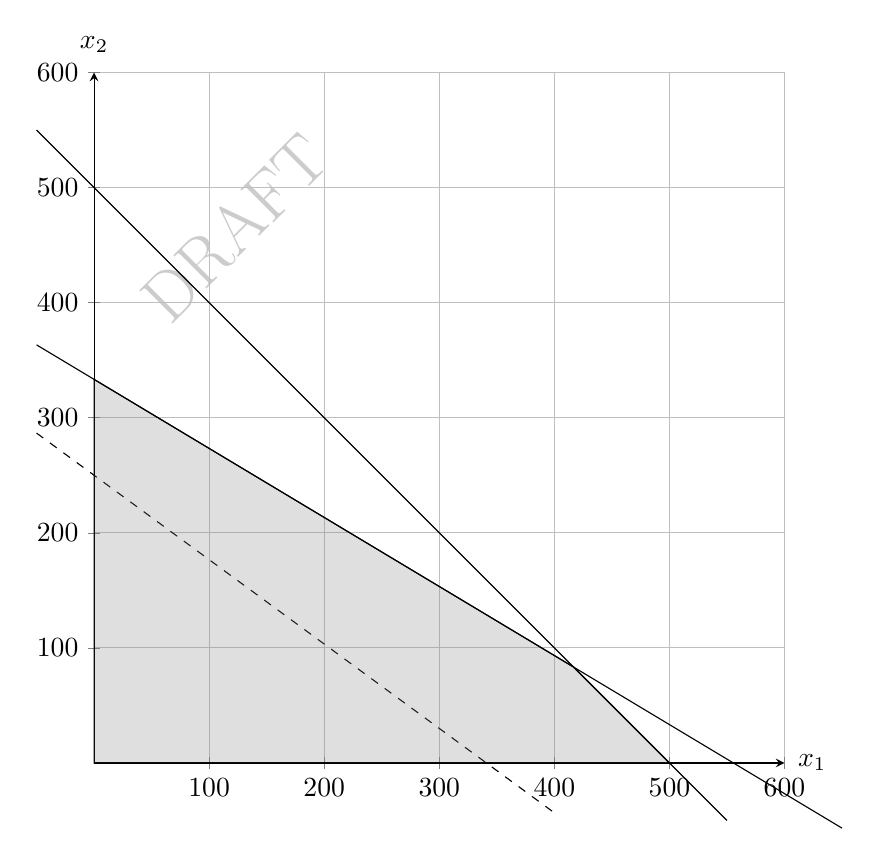
\begin{tikzpicture}
  \begin{axis}[ width=12cm,
    unit vector ratio*=1 1 1,
    enlargelimits=false,
    grid=both,
    axis x line=middle,
    axis y line=middle,
    title=,
    clip=false,
    ymin=0, ymax=600,
    xmin=0, xmax=600]

    \addplot[domain=-50:650] {50000/150 - 90/150*x};
    \addplot[domain=-50:550] {500 - x};
    \addplot[domain=-50:400,dashed] {250 - 110/150*x};
    \addplot[fill=gray, fill opacity=.25]
    coordinates { (0,0) (500,0) (416.67,83.33) (0,333.33) } \closedcycle;

  % to get axis labels at the end of the axis
  \node at (axis description cs:1.04,0) {$x_1$}; \node at
  (axis description cs:0,1.04) {$x_2$};
\end{axis}
\end{tikzpicture}
\end{center}
\caption{Feasible region for the farm problem.}
\label{fig:feasibleregion}
\end{figure}

We now show how to model the farm problem in GAMS.
The complete problem formulation is shown in
figure~\ref{fig:farmer}.

\begin{SaveVerbatim}{vrbfarmer}
variables
x1 'acres of feed corn'
x2 'acres of organic corn'
z;
positive variables x1, x2;

equations
 profit  'objective function'
 budget  'available cash'
 acres   'available acres';

profit.. z =e= 110*x1 + 150*x2;
budget.. 90*x1 + 150*x2 =l= 50000;
acres.. x1 + x2 =l= 500;

model farmer / all /;

solve farmer using LP maximizing z;
\end{SaveVerbatim}

\begin{figure}
\fbox{
\begin{minipage}{\textwidth}
\BUseVerbatim{vrbfarmer}
\caption{Farm problem (\texttt{farmer.gms})}
\label{fig:farmer}
\end{minipage}
}
\end{figure}


Since this problem is small, we include all data parameters directly
in the model specification. However, it is usually good practice to
separate the data from the model, and AMPL encourages this separation
by providing \texttt{param} declarations and the ability to have a
separate \texttt{data} section. We will illustrate these features of
AMPL in the other problem formulations in this article.  AMPL doesn't
actually solve the mathematical programing problem, but rather passes
a description of the problem to a solver, which returns information
about the solution (if any solution was found) to AMPL. An AMPL
session for the forestry problem follows:

\begin{Verbatim}[samepage=true]
ampl: model forester.mod;
ampl: solve;
MINOS 5.5: optimal solution found.
2 iterations, objective 6250
ampl: display x1,x2;
x1 = 25
x2 = 75
\end{Verbatim}

The optimal solution indicates that the forester should harvest 100
acres, but let 25 acres regenerate naturally and plant 75 acres with
pine, for a profit of \$6250. Notice that the entire budget of \$4000
is exhausted because $10 \times 25 + 50 \times 75 = 4000$. When a
resource capacity constraint such as \texttt{acres} or \texttt{budget}
holds with equality in the optimal solution (as in this example), then
the constraint is \emph{binding}; all of the resource associated with
the constraint is being consumed. If more/less of the resource were
available, then profit would be increased/decreased. The value of the
associated dual variable indicates the amount by which profit would be
affected for small changes in the supply of the resource. This is
called the marginal value of a resource, or the shadow price.

\begin{Verbatim}[samepage=true]
ampl: display acres, budget;
acres = 32.5
budget = 0.75
\end{Verbatim}

Displaying the shadow prices in AMPL indicates that an additional acre
of hardwood timber would increase profit by \$32.50, given the same
budget of \$4000.  Modifying the right-hand side of \texttt{acres} to
101 and re-solving shows that this is indeed the case.

\begin{Verbatim}[samepage=true]
ampl: reset;
ampl: model forester.mod;
ampl: expand acres;
subject to acres:
	x1 + x2 <= 101;

ampl: solve;
MINOS 5.5: optimal solution found.
2 iterations, objective 6282.5
ampl: display x1,x2;
x1 = 26.25
x2 = 74.75
\end{Verbatim}

The \texttt{expand} command displays the full form of a set of
constraints.  (This will be useful for indexed expressions.) Notice
that the values of the decision variables have necessarily changed and
that the solution is no longer integer-valued.  This is typical of
resource allocation problems. We are in fact assuming that the
forester is able to execute the decisions on partial acres.  For the
\texttt{budget} constraint, an additional one dollar increase/decrease
in the right-hand side would increase/decrease profit by \$0.75, given
the same 100 acres of hardwood. It stands to reason, then, that the
forester could take out a loan and apply the funds to her
operation. As long as the interest rate is less than .75, profit will
increase.

Shadow prices are valid for \emph{limited} increases/decreases in the
right-hand sides of the constraints. The ranges over which the these
values are valid is a topic of sensitivity analysis. Here, we will
show how to extract this information from AMPL. First we need to tell
AMPL to use a solver that is able to return sensitivity information
along with the optimal solution. We will use the solver
\texttt{cplex}. Then we set a solver-specific option to make the
sensitivity range information available.

\begin{Verbatim}[samepage=true]
ampl: option solver cplex;
ampl: option cplex_options 'sensitivity';
ampl: solve;
CPLEX 11.2.0: sensitivity
CPLEX 11.2.0: optimal solution; objective 6250
2 dual simplex iterations (1 in phase I)

suffix up OUT;
suffix down OUT;
suffix current OUT;
\end{Verbatim}

We are now able to display the ranges over which the current shadow
prices of \$32.5 per acre and \$0.75 per dollar of budget are
valid. To do this we simply add a suffix to the name of the
constraint, separated by a ``\texttt{.}''. The suffix
\texttt{.current} displays the current value of a constraint's
right-hand side, while \texttt{.down} and \texttt{.up} display the
lower and upper limits, respectively. In the AMPL session follows, the
upper limit of 5000 on the right-hand side of \texttt{budget}
indicates the forester should only consider loans of \$1000 or less to
be valued at an incremental marginal value of 0.75.

\begin{Verbatim}[samepage=true]
ampl: display acres.down, acres.current, acres.up;
acres.down = 80
acres.current = 100
acres.up = 400

ampl: display budget.down, budget.current, budget.up;
budget.down = 1000
budget.current = 4000
budget.up = 5000
\end{Verbatim}

Sensitivity ranges may also be obtained for the decision variables. In
this case the lower and upper limits represent the valid ranges on the
objective function coefficients over which the current solution
remains optimal.  The suffix \texttt{.current} refers to the current
value of the coefficient.  Displaying this information for the
forestry problem reveals that the current solution value of \texttt{x1
  = 25} remains optimal as long as its coefficient in the objective
function is in the range 14 to 70, holding all other parameters at
their current values.

\begin{Verbatim}[samepage=true]
ampl: display x1.down, x1.current, x1.up;
x1.down = 14
x1.current = 40
x1.up = 70

ampl: display x2.down, x2.current, x2.up;
x2.down = 40
x2.current = 70
x2.up = 200
\end{Verbatim}

\emph{A Diet Problem.}
Dwight is an elementary school teacher who also raises pigs for
supplemental income. He is trying to decide what to feed his pigs.
Considering a combination of pig feeds available from local suppliers,
he would like to feed the pigs at minimum cost while also making sure
each pig receives an adequate supply of calories and vitamins.  The
cost, calorie content, and vitamin content of each feed are given in
the table below.

\vspace{.1in}
\begin{center}
\begin{tabular}{ccc}
\textbf{Contents}   &  \textbf{Stark County Coop Pig Feed }   & \textbf{Pioneer Pig Feed} \\   \hline
Calories (per pound)  &  800    &  1000   \\
Vitamins (per pound)  &  140 units  &  70 units  \\
Cost (per pound)   &  \$0.40    & \$0.80  \\
\end{tabular}
\end{center}
\vspace{.1in}

Each pig requires at least 8,000 calories per day and at least 700
units of vitamins. A further constraint is that no more than one-third
of the diet (by weight) can consist of Stark County Coop Pig Feed,
since it contains an ingredient which is toxic if consumed in too
large a quantity.  First, let's write down the mathematical
programming formulation without regard to AMPL. Let $x_1$ be the
pounds per day of Stark County Coop feed to purchase. Similarly, let
$x_2$ be the pounds per day of Pioneer feed to purchase. Then the
problem is to 

\[
\begin{array}{lrrrrrl}
\textrm{minimize}   & .4x_1 & + & .8x_2 &  &  &  \\
\textrm{subject to} & 800x_1 & + & 1000x_2 & \geq & 8000 & \textrm{(calories)} \\
                    & 140x_1 & + & 70x_2   & \geq & 700  & \textrm{(vitamins)} \\
					& 2x_1   & - & x_2     & \leq & 0    & \textrm{(toxicity)} \\
\multicolumn{4}{r}{x_1,x_2}& \geq & 0 &
\end{array}.
\]

To get the toxicity restriction on the amount of Stark County Coop
feed, begin with the relation
\[
x_1 \leq \frac{1}{3}(x_1 + x_2).
\]
Then collect terms and simplify.  Since this problem has only two
variables, we can easily specify the model in AMPL by creating each
variable, the objective function, and the three constraints as shown
in Figure~\ref{p1}. This model should be saved in a text file with a
\texttt{.mod} extension.

\begin{SaveVerbatim}{pigs}
var x1 >= 0;  # stark
var x2 >= 0;  # pioneer

minimize total_cost: .4*x1 + .8*x2;

subject to cal: 800*x1 + 1000*x2 >= 8000;
subject to vit: 140*x1 + 70*x2 >= 700;
subject to tox: x1 <= (1/3)*(x1 + x2);
\end{SaveVerbatim}

\begin{figure}
\fbox{
\begin{minipage}{\textwidth}
\BUseVerbatim{pigs}
\caption{AMPL model (\texttt{pigs.mod})}
\label{p1}
\end{minipage}
}
\end{figure}

The following AMPL session shows how to read the problem into AMPL,
invoke the default solver, and print the solution. The minimum cost
feed mixture is 2.86 pounds of Stark County feed and 5.71 pounds of
Pioneer feed per pig per day, for a total cost of \$5.71 per pig per
day.
\begin{Verbatim}[samepage=true]
ampl: model pigs.mod;
ampl: solve;
MINOS 5.51: optimal solution found.
2 iterations, objective 5.714285714
ampl: display x1, x2;
x1 = 2.85714
x2 = 5.71429
\end{Verbatim}

For problems of any reasonable size it is necessary (and desirable) to separate
the model and data. This will allow us to solve different problem instances
(i.e. different sets of data) without changing the model. Figure~\ref{p2} shows
the complete problem formulation and data with separate \texttt{model} and
\texttt{data} sections in the same text file (\texttt{pigs2.mod}). It is also
possible (and you will usually want to do this) to put the data section
in its own text file. In that case we would name the data file with a
\texttt{.dat} extension, e.g. \texttt{pigs2.dat}.

\begin{SaveVerbatim}{pigs2}
model;
set Supplier;

param calories {Supplier};  # per pound
param vitamins {Supplier};  # units per pound
param cost {Supplier};      # dollars per pound

var x {Supplier} >= 0;  # pounds to purchase from each supplier (per pig)

minimize total_cost: sum {i in Supplier} cost[i]*x[i];

s.t. cal: sum {i in Supplier} calories[i]*x[i] >= 8000;
s.t. vit: sum {i in Supplier} vitamins[i]*x[i] >= 700;
s.t. tox: x['stark'] <= (1/3)* sum {i in Supplier} x[i];

data;
set Supplier := stark pioneer;

param : vitamins cost calories:=
stark   140      .4    800
pioneer  70      .8   1000;
\end{SaveVerbatim}

\begin{figure}
\fbox{
\begin{minipage}{\textwidth}
\BUseVerbatim{pigs2}
\caption{Separation of model and data (\texttt{pigs2.mod})}
\label{p2}
\end{minipage}
}
\end{figure}

Most AMPL models are specified by declaring sets, parameters, and
variables, and then by writing the objective function and the
constraints that make use of the sets, parameters, and
variables. Parameters are typically numeric values, although they can
also be logical or symbolic values. They can be thought of as ``data''
values, e.g. the cost per pound of feed. Variables represent the
decisions, e.g. the amount of feed to purchase. Sets specify the
objects with which parameters and variables are associated. We
declared the feed suppliers to be a set because the decisions for how
much feed to purchase as well as cost and nutritional attributes of
the feed are logically associated with each supplier. We say that the
parameters and the variables are \emph{indexed} over the set of
suppliers.

Giving short, meaningful names to sets, parameters, and variables
makes a model readable.  I like to capitalize the first letter of set
names so that they are easily distinguished from parameters.  In the
AMPL book, you will see that set names are in all upper-case
letters. This is just a convention, and the language does not require
it; however, good programming habits will make your code easier to
maintain.

Here is the output from an AMPL session using the model and data in
\texttt{pigs2.mod}.  When working with AMPL, if you read in a model
and subsequently make changes, or if you read in a new model after
having worked with an initial model, you will need to use the
\texttt{reset} command before reading in the new model. Note that when
the decision variables are indexed over a set, we display all of them
at once by typing the variable symbol.
\begin{Verbatim}[samepage=true]
ampl: reset;
ampl: include pigs2.mod;
ampl: solve;
MINOS 5.51: optimal solution found.
2 iterations, objective 5.714285714
ampl: display x;
x [*] :=
pioneer  5.71429
  stark  2.85714
;
\end{Verbatim}

\emph{Factory Planning.}
This example is taken from~\cite{williams:1999}. 
A factory makes seven products that require various amounts of time on four different
types of machines. The factory owns four grinders, two vertical drills, three 
horizontal drills, one boring machine, and one planing machine. 
For each product manufactured, the company can either sell the
product (subject to market limitations) or hold the product in inventory at a cost of
.5 per unit per month. We would like to develop a production and inventory plan for
each of the next six months.
We will not consider the sequence of machine operations; however, there
is a fixed maintenance schedule that specifies when and how many of each machine type
will be unavailable. The factory operates two eight-hour shifts each working day.
There are 24 working days each month.

Refer to the data in figure~\ref{fdat} as well as the model in
figure~\ref{fmod} while reading this description.
Notice that the set \texttt{Month} is declared to be of type \texttt{ordered},
indicating a defined ordering among its (symbolic) members.
This means that we can refer to the members of \texttt{Month} by their relative position.
For example, in our data the expression \texttt{first(Month)} refers
to the member \texttt{'jan'}. One common reason for declaring a set to be \texttt{ordered}
is the need to refer to the previous and/or the next member in an indexed expression.
A typical example of this use of an \texttt{ordered} set is illustrated by the 
\texttt{balance} constraints.

\begin{SaveVerbatim}{vrbfmod}
set Product;
set Machine;
set Month ordered;

param profit {Product} >= 0;
param time_required {Product,Machine} >= 0;
param num_available {Machine} integer, >= 0;
param downtime {Month,Machine} integer, >=0;
param market_limit {Month,Product} integer, >= 0;
param work_hours := 2*8*24;
# number of working hours in a month: 2 shifts of 8 hours each, 24 days/month

var make {Month,Product} >=0;  # how much of each product to make in each month
var sell {Month,Product} >=0;  # how much to sell
var hold {Month,Product} >=0, <=100;  # how much to hold

maximize total_profit:
  sum {t in Month, i in Product} (profit[i]*sell[t,i] - 0.5*hold[t,i]);

s.t. capacity {t in Month, m in Machine}:
sum {i in Product} time_required[i,m]*make[t,i] 
  <= work_hours*(num_available[m]-downtime[t,m]);

s.t. marketing {t in Month, i in Product}: sell[t,i] <= market_limit[t,i];

s.t. balance {t in Month, i in Product : ord(t) > 1}:
  hold[prev(t),i] + make[t,i] = sell[t,i] + hold[t,i];
# on-hand inventory plus number produced must equal number
# sold plus number held in inventory for the next period

s.t. balance0 {i in Product}:
  make[first(Month),i] = sell[first(Month),i] + hold[first(Month),i];
# there is no inventory held over from december

s.t. end_inventory {i in Product}: hold[last(Month),i] = 50;
# stipulate that 50 of each product are to be held over from june
\end{SaveVerbatim}

\begin{figure}
\fbox{
\begin{minipage}{\textwidth}
\BUseVerbatim{vrbfmod}
\caption{Model for factory planning problem (\texttt{factory\_planning1.mod})}
\label{fmod}
\end{minipage}
}
\end{figure}

A defining feature of this model is use of three different variables to represent
the quantities and timing for making, selling, and holding each product.
The relationship among these
variables is stated in the \texttt{balance} constraints.
An upper bound of 100 units on the \texttt{hold} variable represents a storage limitation 
for each product in each month.

Our objective is to maximize the total profit of the factory over a period of six months.
A unit profit is accrued for each item sold and a unit cost of .5 is incurred for each item
held in inventory in a given month.
Note that the parentheses surrounding the subtraction
are necessary because the \texttt{sum} operator has higher precedence than \texttt{-}.
As a side note, if we were to remove the holding cost from consideration in 
the objective then no parentheses would be required around the
\texttt{profit[i]*sell[t,i]} term because the \texttt{sum} operator has lower precedence
than \texttt{*}~\cite{fourer:2003}. 

Each product requires a certain amount of processing time (possibly zero) on each type
of machine. These requirements are specified in the data by the parameter 
\texttt{time\_required} that is indexed over \texttt{Product} and \texttt{Machine}
We need to specify constraints on the amount of machine time
available each month. There are \texttt{work\_hours} production hours available each month
on each machine unless a machine is down for maintenance. Because the maintenance
schedule is specific to each machine and month, the machine capacity constraints 
are indexed over \texttt{Month} and \texttt{Machine}. The total number of machine
hours for all products must not exceed the time available in any particular month
(respecting the \texttt{downtime} schedule.)
There is an upper bound on the amount of each product that the market will absorb
(i.e. that can be sold) each month.

We have three different variables to represent the decisions to make, sell,
and hold product.  The logical relationship among these variables is that
in any particular month the amount sold plus the amount held in inventory
must equal the amount produced plus any inventory from the previous month.
When specifying these product balance constraints we must pay attention to the
boundary conditions when indexing over \texttt{Month}. In our problem, we
cannot refer to the previous month when the dummy index evaluates to \texttt{'jan'}.
We can handle this in the main \texttt{balance} equations by placing a condition
on the indexed set such that the order of the member is greater than 1
(and so \texttt{'jan'} is omitted.)
This is possible because we declared the set \texttt{Month} to be of type
\texttt{ordered}. We then need to specify a separate set of constraints for
the first month (\texttt{balance0}). There is no beginning inventory and 
so the amount produced in \texttt{'jan'} equals the amount sold plus the amount
held.

Instead of using the expression \texttt{make[first(Month),i]},
it would have been legitimate to refer to \texttt{make['jan',i]}; however,
it's better practice to separate the model from the data. The model may then
be applied to other problem instances with the same structure, but perhaps with
a different starting month. Finally, we would like to end June with 50 of
each product type in inventory. This is specified by the equality constraints
named \texttt{end\_inventory}.

\begin{SaveVerbatim}{vrbfdata}
data;
set Product := 1 2 3 4 5 6 7;
set Machine := grinder vdrill hdrill borer planer;
set Month := jan feb mar apr may jun;

param profit := 1 10 2 6 3 8 4 4 5 11 6 9 7 3;

param num_available :=	
grinder 4 vdrill 2 hdrill 3 borer 1 planer 1;

param time_required (tr) :
         1   2   3   4   5   6   7 :=
grinder .5  .7   0   0  .3  .2  .5
vdrill  .1  .2   0  .3   0  .6   0
hdrill  .2   0  .8   0   0   0  .6
borer  .05 .03   0 .07  .1   0 .08
planer   0   0 .01   0 .05   0 .05;

param downtime :
     grinder vdrill hdrill borer planer :=
jan    1       0     0      0     0
feb    0       0     2      0     0
mar    0       0     0      1     0
apr    0       1     0      0     0
may    1       1     0      0     0
jun    0       0     1      0     1;

param market_limit :
       1     2     3     4     5     6     7 :=
jan  500  1000   300   300   800   200   100
feb  600   500   200     0   400   300   150
mar  300   600     0     0   500   400   100
apr  200   300   400   500   200     0   100
may    0   100   500   100  1000   300     0
jun  500   500   100   300  1100   500    60;
\end{SaveVerbatim}

\begin{figure}
\fbox{
\begin{minipage}{\textwidth}
\BUseVerbatim{vrbfdata}
\caption{Data for factory planning problem (\texttt{factory\_planning1.mod})}
\label{fdat}
\end{minipage}
}
\end{figure}

\section{Integer Programming}

\emph{Perfect Matching.}
There are 10 students to be assigned to 5 dorm rooms. Each room holds exactly
two students. For each pair of students, a value that indicates the desirability
of placing that pair in the same room has been determined. Higher values 
correspond to better pairings.
We would like to pair the students in such a way that the
sum total of the values of each assigned pair is maximized. More generally,
the perfect matching problem is to assign $n$ pairs for $2n$ objects (with or without
an objective function). The model and data are presented in figure~\ref{perfect}.

\begin{SaveVerbatim}{vrbperfect}
set Student; 
set Pair within Student cross Student;

param value {Pair};

var x {Pair} binary;

maximize total_value: sum {(i,j) in Pair} value[i,j] * x[i,j];

s.t. perfect_match {i in Student}:
	sum {(i,j) in Pair} x[i,j] + sum {(j,i) in Pair} x[j,i] = 1;

data;
set Student := 1 2 3 4 5 6 7 8 9 10;

param: Pair: value:
   1  2  3  4  5  6  7  8  9 10 :=
1  .  .  .  .  .  .  .  .  .  .
2  3  .  .  .  .  .  .  .  .  .
3  5  8  .  .  .  .  .  .  .  .
4  1 -4  7  .  .  .  .  .  .  .
5  2 -1  9  2  .  .  .  .  .  .
6  2  5  3  2  9  .  .  .  .  .
7  8  2  1  1  3 -2  .  .  .  .
8  2  3  3  4  5  1  1  .  .  .
9 13 -1  3  4  4 -5  2  2  .  .
10 1  2  6  6  7 -4  5  6  1  .;
\end{SaveVerbatim}

\begin{figure}
\fbox{
\begin{minipage}{\textwidth}
\BUseVerbatim{vrbperfect}
\caption{Model and data for perfect matching problem (\texttt{roommates.mod})}
\label{perfect}
\end{minipage}
}
\end{figure}

\texttt{Pair} is a compound set with dimension two. Each member of this set is
an ordered pair of students. We use the term ``ordered'' because the member
(3,7) is distinct from the member (7,3). The \texttt{within} phrase tells
us that the only allowed members in \texttt{Pair} are ordered pairs from the set
\texttt{Student}. Such restrictions in the declaration of sets are encouraged in order to
help detect errors in the data. For example, the following alternative declaration is 
perfectly acceptable, but using it would not allow the AMPL translator to recognize
invalid pairs of students in the data section.
\begin{Verbatim}
set Pair dimen 2;
\end{Verbatim}

The declaration of \texttt{Pair} is not strictly necessary. We could formulate the problem
using only the set \texttt{Student}. However, using the compound set \texttt{Pair}
makes the model easier to read and to maintain, particularly the indexing expressions.
We specify a parameter \texttt{value} that is indexed over \texttt{Pair} to represent the
desirability of matching up a particular pair of students. Our decision variables
\texttt{x} are binary variables that are also indexed over \texttt{Pair}. 
\texttt{x[i,j]} will equal one if student \texttt{i} is matched with student \texttt{j},
and will equal zero otherwise. Notice the \texttt{binary} modifier in the declaration
of \texttt{x}. This means that our decision variables may \emph{only} take on the values zero
or one and turns our formulation into one of pure integer programming~\cite{nemhauser:1988}.

The problem formulation itself consists of the objective function and a single set
of constraints, one for each student. Our objective is to maximize the overall
value of the assignments. It provides a good example of how to iterate over a 
compound set in AMPL. Notice that we must provide a pair of dummy variables
\texttt{(i,j)} to index into \texttt{Pair}. 

The constraints \texttt{perfect\_match} state that each student must be
matched with exactly one other student. To understand how this is 
accomplished note that the scope of the index \texttt{i} extends from 
its introduction in \texttt{i in Student} until the end of the statement
marked by the semi-colon. In the expression \texttt{sum \{(i,j) in Pair\} x[i,j]},
\texttt{i} is held constant for a particular student (row of \texttt{value}) 
and the summation is over all room mates such that the pair of students
represented by \texttt{(i,j)} exist in the set \texttt{Pair}, i.e. the
summation is over columns.
In the second expression with \texttt{i} and \texttt{j} interchanged, the
summation is over rows. This is necessary
due to the way that the data for \texttt{Pair} are structured. Notice that
only the lower left portion of \texttt{value} is filled in.

This example demonstrates how to simultaneously define a set (\texttt{Pair}) and a parameter
(\texttt{value}) that is indexed over that set. The ``\texttt{.}'' symbols indicate
missing values, e.g. there exists no member \texttt{(1,1)} in the set \texttt{Pair}.
An AMPL session for solving this problem follows. Although not strictly necessary
for this particular problem, we will instruct AMPL to use
a solver that can handle integer programming problems, such as the solver
\texttt{gurobi}. 

\begin{Verbatim}[samepage=true]
ampl: option solver gurobi;
ampl: model roommates.mod;
ampl: solve;
Gurobi 3.0.0: optimal solution; objective 39
14 simplex iterations
ampl: display x;
x [*,*]
:    1   2   3   4   5   6   7   8   9    :=
2    0   .   .   .   .   .   .   .   .
3    0   1   .   .   .   .   .   .   .
4    0   0   0   .   .   .   .   .   .
5    0   0   0   0   .   .   .   .   .
6    0   0   0   0   1   .   .   .   .
7    0   0   0   0   0   0   .   .   .
8    0   0   0   1   0   0   0   .   .
9    1   0   0   0   0   0   0   0   .
10   0   0   0   0   0   0   1   0   0
;
\end{Verbatim}

The large number of zeros makes the solution difficult to read. A useful
option is to only display the decision variables with nonzero values. Then
we can easily see that the pairs are (3,2),(6,5),(8,4),(9,1), and (10,7).

\begin{Verbatim}[samepage=true]
ampl: option omit_zero_rows 1;
ampl: display x;
x :=
3  2   1
6  5   1
8  4   1
9  1   1
10 7   1
;
\end{Verbatim}

\emph{Map Coloring.}
The map coloring problem is to assign a color to each area on a map
(e.g. state or county) in such a way that adjacent areas (i.e. those
areas that share a border) are assigned different colors. Moreover, we 
would like to use as few colors as possible. The formulation for this
problem was adapted from code written in GNU MathProg by Andrew
Makhorin~\cite{glpk}.

We may create a representation of the adjacency information by constructing a
graph wherein each area on the map is represented by a node. An 
edge is drawn between two nodes if the respective areas on the map share a border.
As an example, figure ? shows the map and the corresponding
adjacency graph for the western United States. The graph representation
will better facilitate the requirement that adjacent areas must be assigned 
different colors.

\begin{figure}
\begin{center}
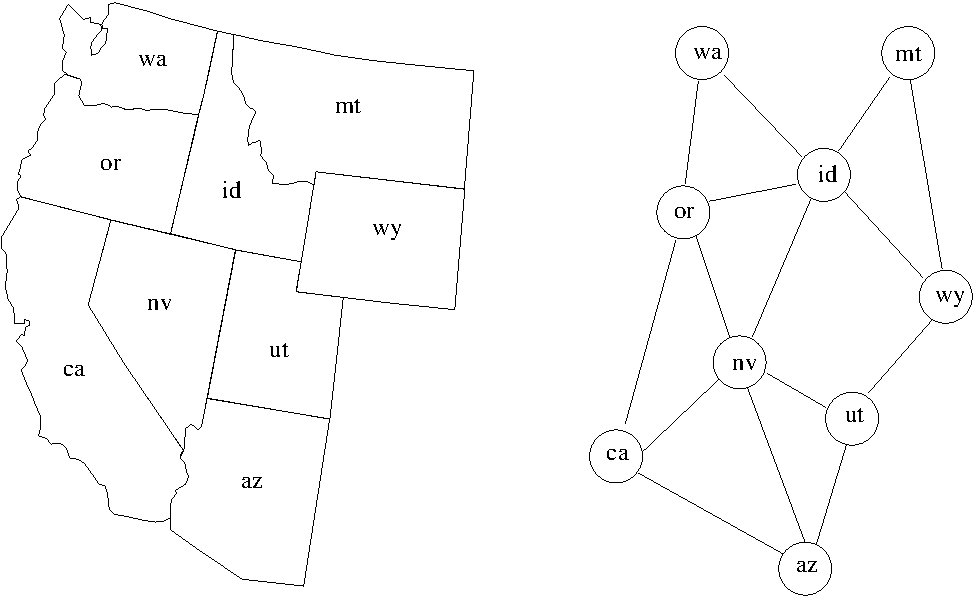
\includegraphics[scale=0.7]{westernusa.pdf}
\caption{Western states and adjacency graph}
\label{westernusa}
\end{center}
\end{figure}

Both the model and the data are presented in figure~\ref{kcolor}. In this model
we must make the cardinality of the set \texttt{Color} large enough to effect
a feasible solution. For a large problem the minimum number of colors needed will not
be obvious (otherwise there is no need to solve the problem.) However, if the 
solver finds that the problem is infeasible we can always add more members to the
set \texttt{Color}. See Andrew Makhorin's code~\cite{glpk} for an implementation
of a heuristic to obtain an upper bound on the required number of colors.

\begin{SaveVerbatim}{vrbkcolor}
set Node;
set Edge within (Node cross Node);
set Color;   
# the cardinality of the set Color needs to be large enough
# to find a feasible solution

var x {Node,Color} binary; # x[i,c] = 1 means that node i is assigned color c
var u {Color} binary;      # u[c] = 1 means that color c is used

minimize num_colors: sum {c in Color} u[c];

s.t. assignment {i in Node}: sum {c in Color} x[i,c] = 1;
# each node is assigned exactly one color

s.t. different {(i,j) in Edge, c in Color}: x[i,c] + x[j,c] <= u[c];
# adjacent nodes must be assigned different colors

data;
set Color := red blue green yellow orange;

set Node := ca or wa mt id nv wy ut az;

set Edge:
   ca or wa mt id nv wy ut az :=
ca -  +  -  -  -  +  -  -  +
or -  -  +  -  +  +  -  -  -
wa -  -  -  -  +  -  -  -  -
mt -  -  -  -  +  -  +  -  -
id -  -  -  -  -  +  +  +  -
nv -  -  -  -  -  -  -  +  +
wy -  -  -  -  -  -  -  +  -
ut -  -  -  -  -  -  -  -  +
az -  -  -  -  -  -  -  -  -;
\end{SaveVerbatim}

\begin{figure}
\fbox{
\begin{minipage}{\textwidth}
\BUseVerbatim{vrbkcolor}
\caption{Model and data for map coloring problem (\texttt{kcolor.mod})}
\label{kcolor}
\end{minipage}
}
\end{figure}

Our binary decision variables \texttt{x} will indicate the particular color 
assigned to each node (area on the map). We also create binary modeling variables
\texttt{u} to indicate that a color has been used in the solution. Now the
objective is a simple summation over \texttt{u}. There are three dummy variables
in the indexing expression for the \texttt{different} constraint. Notice
that even though \texttt{x} is indexed over \texttt{\{Node,Color\}} the
indexing expression for \texttt{different} will only create one constraint for
each existing \texttt{Edge} and \texttt{Color} combination. Since \texttt{Edge}
is declared to be \texttt{within (Node cross Node)} we may safely use the
dummy indices \texttt{i} and \texttt{j} when indexing into \texttt{x}.

In the \texttt{data} section we see one way to specify the members of a 
two-dimensional set: the ``\texttt{+}'' symbols indicate membership while the
``\texttt{-}'' symbols indicate non-membership. Alternatively, we could have
specified \texttt{Edge} by providing only the ordered pairs.
\begin{Verbatim}[samepage=true]
set Edge :=
(ca,or)   (ca,az)   (or,id)   (wa,id)   (mt,wy)   (id,wy)   (nv,ut)   (wy,ut)
(ca,nv)   (or,wa)   (or,nv)   (mt,id)   (id,nv)   (id,ut)   (nv,az)   (ut,az);
\end{Verbatim}

\section{Dynamic Programming}

\section{Inventory Models}

\clearpage
\section{Exercises}
\begin{enumerate}

% written by Hannah
\item \emph{Feasible region for an LP.} Indicate graphically whether each of the following
  linear programs has a feasible solution. Graphically determine the
  optimal solution, if one exists, or show that no optimal solution
  exists.

\begin{enumerate}
\item
\[
  \begin{array}{lrrrrr}
    \textrm{maximize}   & x_1& +& 3x_2&  & \\
    \textrm{subject to} & x_1& -&4x_2& \leq & 4  \\
                        & x_1& +& 2x_2& \leq & 4 \\
    \multicolumn{3}{r}{x_1,x_2}&       \geq & 0 
  \end{array}
\]

\item
\[
  \begin{array}{lrrrrr}
    \textrm{minimize}   & x_1& +& 2x_2&  & \\
    \textrm{subject to} & 2x_1& -&x_2& \leq & 3  \\
                        & 2x_1& -& x_2& \geq & -3 \\
    \multicolumn{3}{r}{x_1,x_2}&       \geq & 0 
  \end{array}
\]

\end{enumerate}

\begin{solution}
\bs The feasible region for the linear program in part a) is shown
below. The objective function is plotted as a dashed line. The
optimal solution occurs at $x_1=0$, $x_2=2$, and value of the
objective function at the optimal solution is $z=6$.

\begin{center}
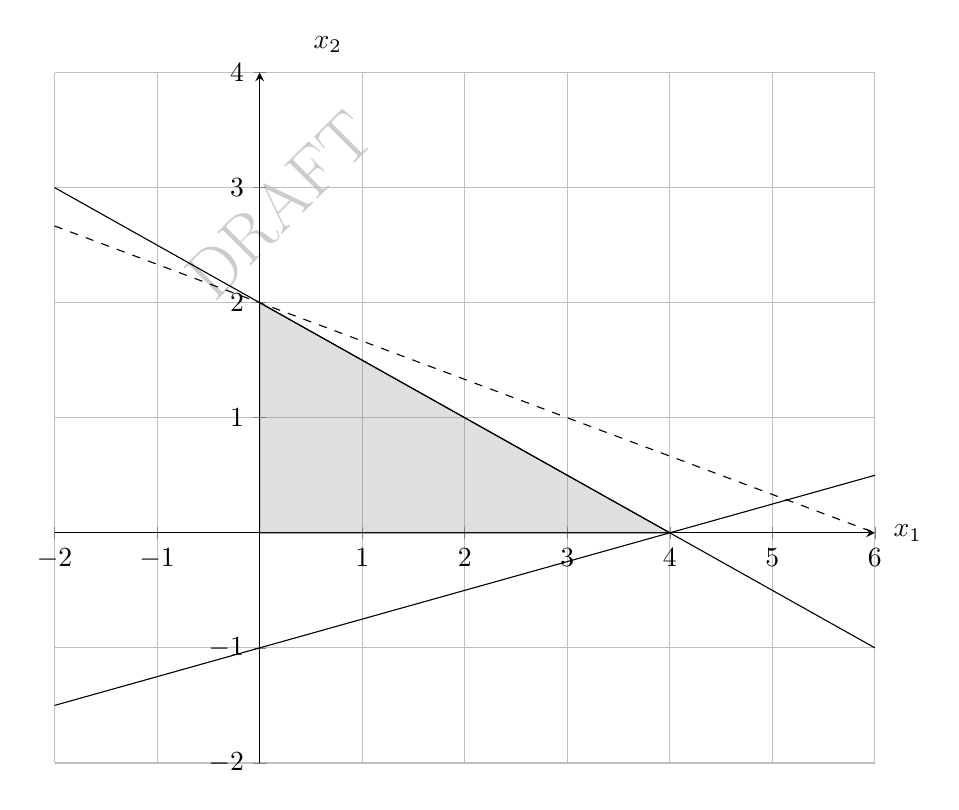
\begin{tikzpicture}
  \begin{axis}[ width=12cm, grid=both, axis x line=middle, axis y
    line=middle, title=, clip=false, ymin=-2, ymax=4, xmin=-2,
    xmax=6 ]

    \addplot[domain=-2:6] {-1 + 1/4*x}; \addplot[domain=-2:6] {2
      - 1/2*x}; \addplot[domain=-2:6,dashed] {2 - 1/3*x};
    \addplot[fill=gray, fill opacity=.25] coordinates { (0,0)
      (4,0) (0,2) }\closedcycle;

    % to get axis labels at the end of the axis
    \node at (axis description cs:1.04,.333) {$x_1$}; \node at
    (axis description cs:.333,1.04) {$x_2$};
  \end{axis}
\end{tikzpicture}
\end{center}

The feasible region for the linear program in part b) is unbounded;
however, since it is a minimization problem, it has an optimal
solution at $x_1=0$, $x_2=0$. The value of the objective function at
the optimal solution is $z=0$.

\begin{center}
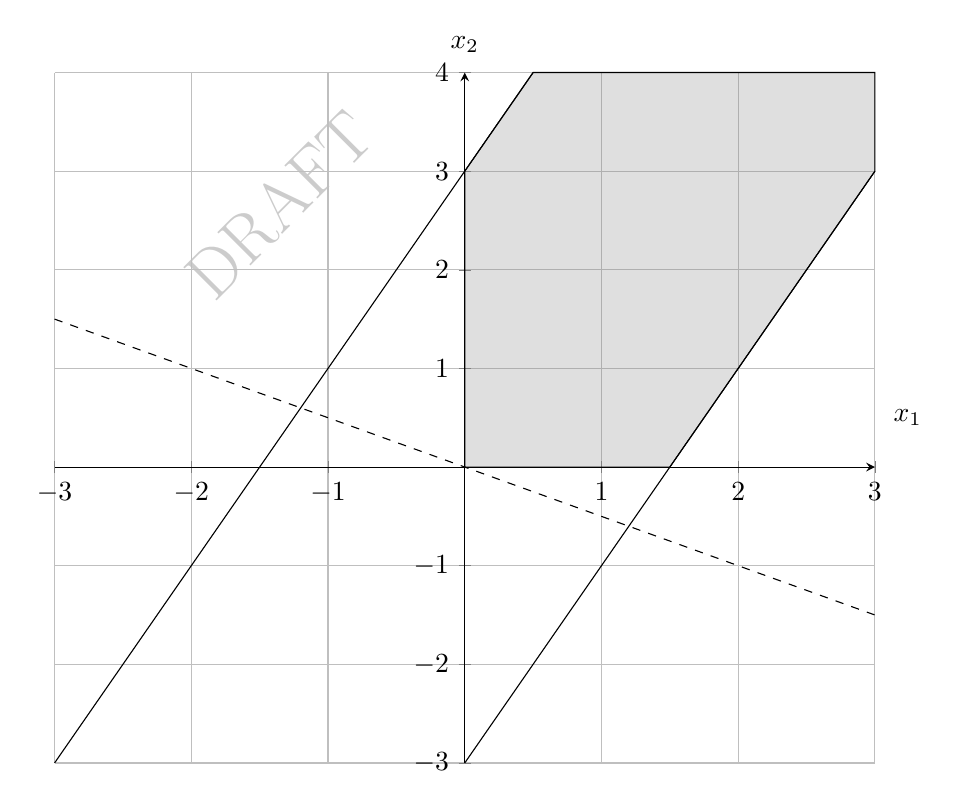
\begin{tikzpicture}
  \begin{axis}[ width=12cm, grid=both, axis x line=middle, axis y
    line=middle, title=, clip=false, ymin=-3, ymax=4, xmin=-3,
    xmax=3 ]

    \addplot[domain=0:3] {-3 +2*x}; \addplot[domain=-3:.5] {3+2*x};
    \addplot[domain=-3:3,dashed] {-1/2*x}; \addplot[fill=gray, fill
    opacity=.25] coordinates { (0,0) (0,3) (.5,4) (3,4) (3,3) (1.5,0)
    }\closedcycle;

    % to get axis labels at the end of the axis
    \node at (axis description cs:1.04,.5) {$x_1$}; \node at (axis
    description cs:.5,1.04) {$x_2$};
  \end{axis}
\end{tikzpicture}
\end{center}

\end{solution}

% re-written by Hannah
\item \emph{Karl's garden.}
Karl is a local gardener who grows lettuce, broccoli, and carrots. His garden is 
400 ft$^2$, and each individual plant of lettuce, broccoli, and carrots occupies 
0.5 ft$^2$, 1.2 ft$^2$, and 0.25 ft$^2$, respectively. Karl recently learned that 
many of his neighbors are interested in purchasing his vegetables. After polling the 
neighborhood, he learned that he has demand for 350 lettuce plants, 350 broccoli plants, 
and 250 carrot plants. Karl estimates that he will earn a profit of \$9.50 per 
lettuce plant, \$12.80 per broccoli plant, and \$8.25 per carrot plant. How many 
plants of each type of vegetable should Karl grow to maximize profit? Solve this 
problem using optimization software.

\begin{solution}
  \bs A GAMS model is provided in the file
  \texttt{karls-garden.gms}. The solution indicates that Karl should
  grow 350 lettuce plants, 135 broccoli plants, and 250 carrot plants
  for a total profit of about \$\num{7120}. Note that we are ignoring
  any fractional values of the decision variables.
\end{solution}


% this problem needs to be re-written, but I think we can just
% change the context and leave the numbers as they are (or very close
% anyway). the idea is to extract a shadow price and use it
% to answer questions.
\item \emph{Workplace safety.}  A manufacturing
  company has assembled a safety committee to reduce the number of
  injuries sustained by employees at work. The company has allotted
  the committee a budget of \$100 each week for purchasing items that
  will increase employee safety. After analyzing past incidents, the
  safety committee has concluded that the most common work hazard is
  exposure to loud noises. As a result, the committee would like to
  purchase (i) earplugs and (ii) other PPE (personal protection
  equipment). The relative value (utility) of the safety items was
  investigated, and it was determined that earplugs provide 1.2 units
  of value for each dollar spent on other types of PPE. The safety
  committee would like to determine how to spend the budget to
  maximize the safety of employees, but the company does not want to
  spend more than \$70 on earplugs and \$50 on other PPE each
  week. The committee also has the option to save part of the money.
  Additionally, the company would like to know:
\begin{enumerate}
\item How the total value of its expenditures for safety would change
  if there were only \$99 to spend. \label{safetya}
\item How the total value would change if \$75 could be spent on
  earplugs.\label{safetyb}
\item Whether it would save any money if each dollar of savings would
  provide 1.1 units of value for each dollar spent on other
  PPE.\label{safetyc}
\end{enumerate}
Formulate the safety committee's spending decision as a linear program. Sketch
the feasible region and determine the optimal solution using the
graphical method.  Then solve the linear program using optimization
software and obtain post-optimality output (i.e. a sensitivity
report).  Use this output to answer each of the questions \ref{safetya},
\ref{safetyb}, \ref{safetyc}.

\begin{solution}
\bs In the problem formulation to maximize total value, let
\[
  \begin{array}{lcl}
    x_1 &=& \textrm{\$ to spend on earplugs} \\
    x_2 &=& \textrm{\$ to spend on other PPE}
  \end{array}
\]
Then the committee wants to solve the following problem.
\[
\begin{array}{lrrrrr}
\textrm{maximize}   & 1.2x_1& +& x_2&      &   \\
\textrm{subject to} & x_1& +&x_2& \leq & 100 \\
                    & x_1& & & \leq & 70 \\
                    & & & x_2& \leq & 50 \\
\multicolumn{4}{r}{x_1,x_2}&       \geq & 0
\end{array}
\]

The feasible region is given below. The optimal solution is $x_1=70$ and $x_2=30$
for a total value of 114.
\begin{center}
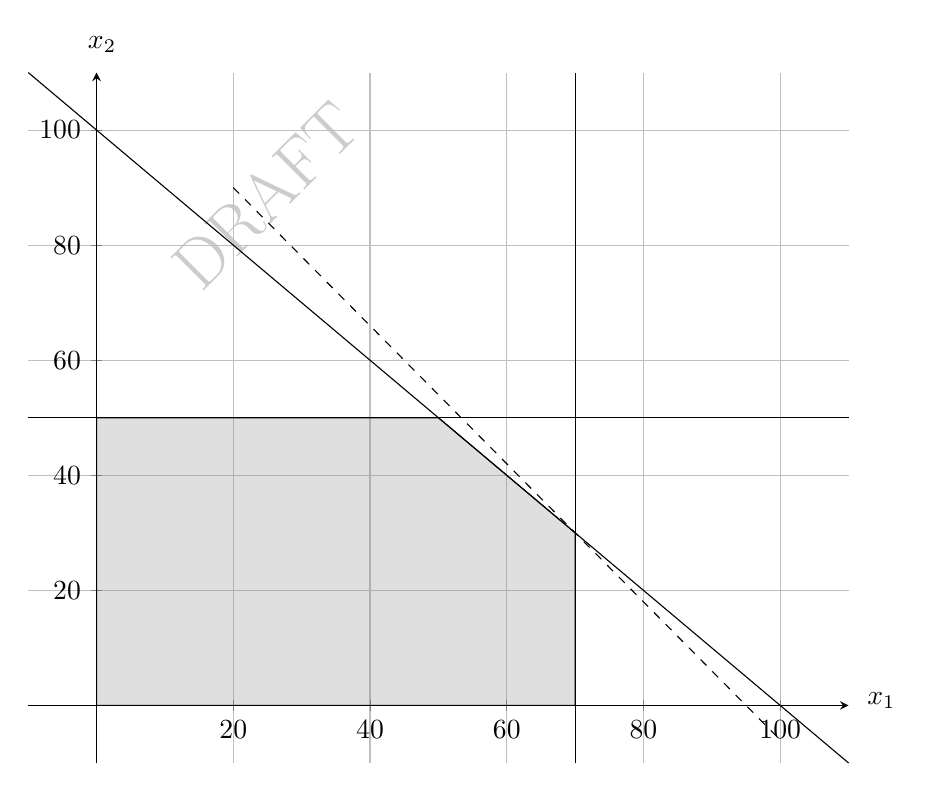
\begin{tikzpicture}
  \begin{axis}[ width=12cm, grid=both,
    axis x line=middle,
    axis y line=middle,
    title=, clip=false,
    ymin=-10, ymax=110, xmin=-10, xmax=110 ]

    \addplot[domain=-10:110] {-x + 100};
    \addplot[mark=none] coordinates {(70,-10) (70,110)};
    \addplot[domain=-10:110] {50};
    \addplot[fill=gray, fill opacity=.25] coordinates {
      (0,0) (70,0) (70,30) (50,50) (0,50) }\closedcycle;
    \addplot[domain=20:100,dashed] {-1.2*x + 114};

    % to get axis labels at the end of the axis
    \node at (axis description cs:1.04,.09) {$x_1$};
    \node at (axis description cs:.09,1.04) {$x_2$};
  \end{axis}
\end{tikzpicture}
\end{center}

A GAMS model is provided in \texttt{workplace-saftey.gms}. Refer to
the listing file \texttt{workplace-saftey.lst}, to answer questions
\ref{safetya}, \ref{safetyb}, and \ref{safetyc}.  Regarding part
\ref{safetya}, the shadow price on the \texttt{budget} constraint
tells us that if we decrease the RHS from 100 to 99, the value of the
objective function will decrease to 113. Since earplugs provide more
value than other PPE, the new solution will be $x_1=70$ and $x_2=29$.
For part \ref{safetyb}, notice that \$75 is within the range for the
shadow price on the \texttt{earplugs} constraint. So, increasing the
RHS to 75 will increase the total value by
\[ \$5 \times 0.2~\text{units of value per dollar} = 1 \]
for a total value of 115.
Finally, for part \ref{safetyc}, saving one dollar requires \$1; however, the
company gets 1.1 units of value for each dollar saved. Yes, the
company would save \emph{some} amount of money and spend less on other
PPE. To use the shadow price to answer this question, notice that the
shadow price on the \texttt{budget} constraint is 1. If we
``price-out'' the new activity of saving money, we see that it cost
\$1 per unit, but it returns \$1.1 per unit in total value. So the
company would save some amount of money. The question did not ask us
to determine the new solution. It only asked whether \emph{any} money
would be allocated to savings.
\end{solution}

% this problem needs to be re-written and GAMS code added.
\item \emph{A blending problem.}  A pet food manufacturer is
  developing a new dog food recipe with natural ingredients. It has
  been decided that the recipe will contain a combination of 4
  ingredients: chicken, brown rice, vegetables, and corn meal. The
  cost and important nutritional information for each ingredient is
  summarized in the table below.

\begin{center}
\begin{tabular}{lcccc} \\
Ingredient  &   Cost (\$/lb)  & Protein (g/lb)  &  Fat (g/lb) &  Fiber (g/lb)  \\ \hline
(1) Chicken   &  3.00 & 125 & 60 & 0 \\
(2) Brown rice   &  0.75 & 12 & 4 & 9 \\
(3) Vegetables   &  1.80 & 14 & 1.5 & 12 \\
(4) Corn meal& 0.60 & 32 & 8 & 17
\end{tabular}
\end{center}

Industrial engineers have been asked to determine the most
cost-effective mixture of ingredients given the following guidelines:
\begin{itemize}
\item Each pound of dog food must contain less than 40 grams of fat
\item Each pound of dog food must contain at least 80 grams of protein 
\item Each pound of dog food must contain between 4 and 10 grams of fiber
\item Each ingredient must comprise at least 10\% of the mixture
\end{itemize}

\begin{enumerate}
\item Formulate an (algebraic) mathematical programming model using
  the information above and generate a solution using software.
  \label{doga}

\item Formulate an alternative (algebraic) mathematical programming
  model given the additional constraint that 80\% of the mixture must
  contain a combination of chicken and vegetables. Generate a solution
  using software and determine the added cost due to the new
  constraint. \label{dogb}
\end{enumerate}

\begin{solution}
\bs For part \ref{doga}, a GAMS model is provided in the file \texttt{dog-fooda.gms}.
The mixture should contain 55.7\% chicken, 10\% brown rice, 10\% vegetables, and 24.3\% corn meal for a cost of \$2.07 per pound.
	
For part \ref{dogb}, A GAMS model is provided in
\texttt{dog-foodb.gms}. The added cost due to the additional
constraint is \$0.20. The mixture should contain 58\% chicken, 10\%
brown rice, 22\% vegetables, and 10\% corn meal for a cost of \$2.27
per pound.
\end{solution}


% re-written by Hannah
\item \emph{Golf lessons.}  Amy and Brian are professional
  golfers who have each agreed to donate 10 hours of private golf
  lessons to a charity auction. Three people have bid on the lessons,
  and their bids are shown in the table below. For example, Emma has
  bid \$28 per hour to receive lessons from Amy.

\begin{tabular}{lrr}
Bidder & Amy & Brian \\ \hline
Emma & \$28/hr & \$30/hr \\
Dan     & \$26/hr & \$28/hr \\
Sam  & \$30/hr & \$32/hr
\end{tabular}

In the spirit of fairness, the auction committee has decided that no bidder can win 
more than 8 hours of total instruction. Given the bid amounts, the committee must now
decide how to allocate the 20 hours of available instruction time.
\begin{compactenum}
  \item Draw a diagram of the problem as a network flow model.
  \item Formulate a linear programming model to maximize the
    charity's revenue.
  \item Solve the problem using optimization software.
\end{compactenum}

\begin{solution}
  \bs A diagram of the network flow model is shown below. Bidders 1, 2,
  and 3 correspond to Emma, Dan, and Sam, respectively.
\vspace{.2in}
\begin{center}
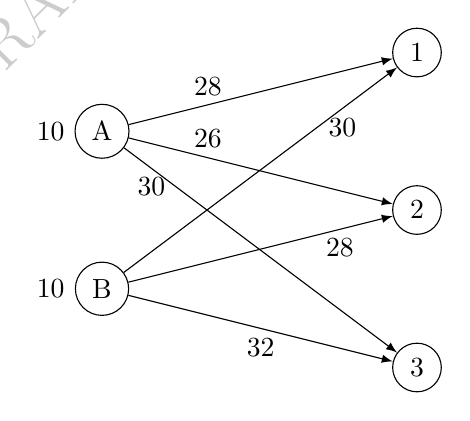
\begin{tikzpicture}[>=latex] % to get latex arrowheads

  \node[circle,draw](B) at (0,2) {B};
  \node[circle,draw](A) at (0,4) {A};
  \node[circle,draw](3) at (4,1) {3};
  \node[circle,draw](2) at (4,3) {2};
  \node[circle,draw](1) at (4,5) {1};

  \draw[->] (A) -- (1) node[above,pos=.3]{28};
  \draw[->] (A) -- (2) node[above,pos=.3]{26};
  \draw[->] (A) -- (3) node[below,pos=.1]{30};
  \draw[->] (B) -- (1) node[below,pos=.8]{30};
  \draw[->] (B) -- (2) node[below,pos=.8]{28};
  \draw[->] (B) -- (3) node[below,pos=.5]{32};

  \node[anchor=east] at (A) {10~~~~};
  \node[anchor=east] at (B) {10~~~~};

\end{tikzpicture}
\end{center}

Let $x_{ij}$ be the number of hours of instruction bidder $j$ receives
from professional golfer $i$.
  \[
     i \in \{\text{A},\text{B}\} \qquad j \in \{1,2,3\}
  \]
  The problem formulation is
\[
  \begin{array}{lrrrrrrrrrr}
    \textrm{maximize} &&&&&&&&&&\\   
    28x_{\text{A}1}&+& 26x_{\text{A}2}&+&30x_{\text{A}3}&+&30x_{\text{B}1}&+&28x_{\text{B}2}&+&32x_{\text{B}3} \\ \\
    \textrm{subject to}  &&&&&&&&&&\\
    & & & & x_{\text{A}1}&+ & x_{\text{A}2}&+ &x_{\text{A}3} & = & 10 \\
    & & & & x_{\text{B}1}&+ & x_{\text{B}2}&+ &x_{\text{B}3} & = & 10 \\
    & & & & & &  x_{\text{A}1} & + & x_{\text{B}1} & \leq & 8 \\
    & & & & & &  x_{\text{A}2} & + & x_{\text{B}2} & \leq & 8 \\
    & & & & & &  x_{\text{A}3} & + & x_{\text{B}3} & \leq & 8 \\
    \multicolumn{11}{r}{x_{ij} \geq 0 \quad \text{for}~i \in \{\text{A},\text{B}\},~j \in \{1,2,3\} }
  \end{array}
\]

The optimal solution is: bidder 1 (Emma) receives 6 hours of
instruction with Amy and 2 hours of instruction with Brian, bidder 2
(Dan) receives 4 hours of instruction with Amy, and bidder 3 (Sam)
receives 8 hours of instruction with Brian. The charity receives \$588
in revenue. A GAMS model and solution is provided in
\texttt{golf-lessons.gms}.  \emph{Note:} There are multiple optimal
solutions to this problem, so the values of the decision variables in
your solution could differ, but the value of the objective function
will be the same.
\end{solution}

% integer programming
% this problem need to be re-written.
% the idea is that it is a set covering problem.
\item \emph{A set covering problem.}  A general merchandise retailer
  is planning to expand into a new metropolitan area comprised of
  seven cities. The following table shows the distance (in miles)
  between each city.

\begin{center}
\begin{tabular}{l|ccccccc}
& \multicolumn{7}{c}{To} \\
From & City 1 & City 2 & City 3 & City 4 & City 5 & City 6 & City 7\\ \hline
City 1 & 0 & 15 & 20 & 38 & 20 & 28 & 22 \\
City 2 & 15 & 0 &  5 & 23 & 16 & 12 & 10 \\
City 3 & 20 & 5 & 0 & 18 & 12 & 13 & 14 \\
City 4 & 38 & 23 & 18 & 0 & 31 & 19 & 27 \\
City 5 & 20 & 16 & 12 & 31 & 0 & 7 & 19 \\
City 6 & 28 & 12 & 13 & 19 & 7 & 0 & 22 \\
City 7 & 22 & 10 & 14 & 27 & 19 & 22 & 0 \\
\end{tabular}
\end{center}

The company assumes that customers will only visit a retail location
if it is within 15 miles of the city in which the customer
lives. Using this information, the company would like to construct the
fewest number of stores while ensuring that they can serve every
customer in the metropolitan area. Formulate an integer programming
model to determine the cities where retail locations should be
constructed.

\begin{solution}
\bs
\begin{equation*}
\text{Let $x_i$} = 
\begin{cases}
  1 & \text{if a retail location is constructed in city $i$,}\\
  0 & \text{otherwise.}
\end{cases}
\end{equation*}

To model the requirement that there is at least one retail location within
15 miles of city 1, we require that $x_1 + x_2 \geq 1$. The full
problem formulation is
\[
\begin{array}{lrrrrrrrrrrrrl}
\textrm{minimize} & \sum_{i=1}^{7} x_i & & & & & & \\
\textrm{subject to} && & & & & & & & x_1 & + & x_2 & \geq & 1 \\
& & & x_1 & + & x_2 & + & x_3 & + & x_6 & + & x_7 & \geq & 1 \\ & &  & x_2 & + & x_3 & + & x_5 & + & x_6 & + & x_7 & \geq & 1 \\
& &  & & & & & &  &  &  & x_4 & \geq & 1 \\
& & & &  & &  & x_3 & + & x_5 & + & x_6 & \geq & 1 \\
& & & &  & x_2 & + & x_3 & + & x_5 & + & x_6 & \geq & 1 \\
& & & & & & & x_2 & + & x_3 & + & x_7 & \geq & 1 \\
\multicolumn{14}{r}{x_i \in \{0,1\} \quad i = 1,\ldots,7}
\end{array}
\]
\end{solution}

% integer programming with a fixed charge
% this problem needs to be re-written.
% i like the idea of renting machinery if an activity is undertaken.
% maybe an example of bicycle manufacturing ...
% types are mountain bike, road bike, fat bike, each requires a different machine.
% resources are labor and material (e.g. aluminum.)
\item \emph{A problem with a fixed charge.}  A bicycle manufacturing
  company can produce three types of bikes: mountain bikes, road
  bikes, and fat bikes. The company rents specific machinery for
  producing each type of bike. It costs \$150 per week to rent
  machinery for mountain bikes, \$250 per week to rent machinery for
  road bikes, and \$300 per week to rent machinery for fat bikes. A
  maximum of 120 hours of labor and \num{11000} pounds of material
  (aluminum) are available each week for production. The material
  and labor requirements to produce one unit of each type of bike are
  shown in the table below. The unit variable cost and the unit
  selling price for each type of bike are also shown.

\vspace{.1in}
\begin{tabulary}{5.4in}{LRRRR}
& Labor (hours) 
& Material (pounds) 
& Variable cost 
& Selling price \\ \hline
Mtn bike & 2.5 & 28 & \$350 & \$550 \\
Road bike & 7 & 25 & \$420 & \$800 \\
Fat bike & 4.5 & 36 & \$680 & \$\num{1200}
\end{tabulary}
\vspace{.1in}

The machinery needed to produce a specific type of bike is only rented
if that type of bike is produced. Assume that the company can sell all
of the bikes that it produces, regardless of type.  Formulate a mixed
integer linear programing problem to determine the weekly production
quantities of mountain bikes, road bikes, and fat bikes that will
maximize profit.

\begin{solution}
  \bs Let the decision variables $x_1,x_2,x_3$ be the number of
  mountain bikes, road bikes, and fat bikes, respectively, to produce
  each week. Machinery rental costs are only incurred if bicycles of that
  particular type are produced. We introduce binary decision variables
  $y_i$ to apply the machinery rental costs when production $x_i$ is
  positive.
\[
\text{Let $y_i$} = 
\begin{cases}
1 & \text{if $x_i > 0$} \\
0 & \text{otherwise}
\end{cases}
\quad i = 1,2,3.
\]
The mathematical formulation of the Integer Programming problem is
\[
\begin{array}{lrrrrrrl}
\textrm{maximize} &   & 550x_1 & + & 800x_2 & + & \num{1200}x_3 & \\
& - & 350x_1  & - & 420x_2 & - & 680x_3  & \\
& - & 150y_1& - & 250y_2&- & 300y_3& \\
& & & & & & &\\
\textrm{subject to} & 2.5x_1 & + & 7x_2 & + & 4.5x_3 & \leq & 120 \\
& 28x_1 & + & 25x_2 & + & 36x_3 & \leq & \num{11000} \\
& & & & & x_1 & \leq & My_1 \\
& & & & & x_2 & \leq & My_2 \\
& & & & & x_3 & \leq & My_3 \\
\end{array}
\]
where $M$ is a large number, $x_i \geq 0$, $x_i$ are integer-valued, 
$y_i \in \{0,1\}$, and $i = 1,2,3$.
\end{solution}

% this problem needs to be re-written. it is problem 5 of ch 10 in IMS.
\item \emph{Ordering diesel fuel.} The Metropolitan Bus Company (MBC)
  purchases diesel fuel from American Petroleum Supply. In addition to
  the fuel cost, American Petroleum Supply charges MBC \$250 per order
  to cover the expenses of delivering and transferring the fuel to
  MBC' s storage tanks. The lead time for a new shipment from American
  Petroleum is 10 days; the cost of holding a gallon of fuel in the
  storage tanks is \$0.04 per month, or \$0.48 per year; and annual
  fuel usage is \num{150000} gallons. MBC buses operate 300 days a
  year.

\begin{enumerate}
\item What is the optimal order quantity for MBC?
\item How frequently should MBC order to replenish the gasoline
  supply?
\item The MBC storage tanks have a capacity of 15,000 gallons. Should
  MBC consider expanding the capacity of its storage tanks? \label{ex:tankcap}
\item What is the reorder point?
\end{enumerate}

\begin{solution}
\bs The cost per order is $C_0=\$250$, the holding cost is
$C_h=\$.48$ per gallon per year, the lead time is $m=10$ days, the
demand rate is $D=\num{150000}$ gallons per year, and there are 300
working days per year. Using the formula for economic order quantity,
\[ Q^{\ast} = \sqrt{\frac{2DC_o}{C_h}} = \sqrt{\frac{2(\num{150000})(250)}{.48}} = \num{12500}~\text{gallons.} \]

The cycle time associated with the economic order quantity is
\[ T^{\ast} = \frac{Q^{\ast}}{D} = \frac{\num{12500}}{\num{150000}\frac{1~\text{year}}{300~\text{days}}} = 25~\text{days.} \]

Regarding part~\ref{ex:tankcap}, the answer is no, because the optimal
order quantity $Q^{\ast}=\num{12500}$ is less than the storage
capacity of \num{15000} gallons.

With 10 days lead time and usage rate of 500 gallons per day, the reorder
point is $10 \times 500 = \num{5000}$ gallons.
\end{solution}



\end{enumerate}

\chapter{Probabilistic Modeling}

\section{Modeling with Probability Distributions}

% use this section to illustrate modeling with a poisson rv
At a facility that manufactures recreational sports
  vehicles (ATVs), each vehicle is subjected to a final
  inspection. The rate of defects during final inspection is
  $\lambda=1.5$ defects per vehicle.
\begin{enumerate}
\item What is an appropriate probability distribution to model the
number of defects? \label{atv1}
\item What proportion of vehicles have more than 2 defects? \label{atv2}
\item Management has set a new goal that the proportion
of vehicles with no defects is .5. What rate $\lambda$ would
achieve this goal? \label{atv3}
\end{enumerate}

We are interested in the number of defects, which is discrete.
The Poisson distribution makes sense because it is commonly used
for count data. Moreover, we are given information for a single
parameter, and the Poisson distribution has a single parameter.
If we let the random variable $X$ represent the number of defects
per vehicle, then a reasonable distribution is
\[ X \sim \text{Poisson}(\lambda=1.5) \]
For part~\ref{atv2},
\begin{align*}
P(X>2) &= 1 - P(X \leq 2)\\
       &= 1 - \sum_{x=0}^2 \frac{e^{-\lambda}\lambda^x}{x!}\\
       &= 0.191
\end{align*}
For part \ref{atv3}, management's goal is that $P(X=0)=0.5$, or
\[ P(X=0) = \frac{e^{-\lambda}\lambda^0}{0!} = e^{-\lambda}=0.5 \]
Then
\[ \lambda = -\ln{0.5} = 0.693 \]

% discussion on the Normal distribution
A refinery makes two grades of gasoline, regular and premium.  The
advertised octane ratings are 87 for regular gasoline and 89 for
premium gasoline.  The quality engineer at the refinery asks for 10
samples from one of the two types of gasoline. She does not know for
sure whether the samples are from the regular batch or the premium
batch. She devises the hypothesis test
\begin{align*}
H_0: \mu &\leq 87 \\
H_1: \mu &> 87
\end{align*}
and sets the confidence level to be 0.995. Suppose that the mean of
the 10 samples is 88.3 and the standard deviation is 1.0. What is her
conclusion for the hypothesis test?

Suppose that a gas station owner has his own octane test
kit and rule for accepting a tanker-truck of premium gasoline.
The owner knows from past shipments that the distributions
of octane ratings are
\begin{align*}
X_{\text{regular}} &\sim N(87,1) \\
X_{\text{premium}} &\sim N(89,1)
\end{align*}
Although the owner may not think about it explicitly, his hypothesis
test is
\begin{align*}
H_0: \mu &= 87 \\
H_1: \mu &= 89
\end{align*}
The owner takes one sample from the tanker-truck. If the octane
measurement is greater than 88.5, then he will accept the shipment as
premium gasoline. What is the probability that the owner accepts a
shipment of regular gasoline as premium (i.e. what is $\alpha$)? What
is the probability that he declines a shipment of premium gasoline,
claiming that he thinks it is regular (i.e. what is $\beta$)?  Use the
Normal distribution for this problem. The following diagram may help.

\begin{tikzpicture}
\begin{axis}[
  no markers, domain=0:12, samples=100,
  height=5cm, width=15cm,
  axis x line=bottom,
  axis y line=none,
  xtick=\empty, ytick=\empty,
  extra x ticks={4,6,7},
  extra x tick labels={87,88.5,89},
  enlargelimits=false, clip=false
  ]
  
  \addplot [fill, pattern=north west lines, domain=0:6] {gauss(7,1)} \closedcycle;
  \addplot [fill, draw=none, domain=6:12] {gauss(4,1)} \closedcycle;
  \addplot [thick] {gauss(4,1)};
  \addplot [thick] {gauss(7,1)};

  \draw [ultra thin] (4,0) -- (4,.3989);
  \draw [ultra thin] (7,0) -- (7,.3989);

  \draw (4,.42) node[anchor=south] {$H_0$};
  \draw (7,.42) node[anchor=south] {$H_1$};

  \draw (4.9,.15) node[anchor=east] (beta) {$\beta$};
  \draw (5.4,.03) node (beta2) {};
  \draw[-] (beta) -- (beta2);

  \draw (6.5,.15) node[anchor=west] (alpha) {$\alpha$};
  \draw (6.1,.005) node (alpha2) {};
  \draw[-] (alpha) -- (alpha2);
  
\end{axis}
\end{tikzpicture}

For the quality engineer, the test statistic is
\[
t_0 = \left( \overline{X} - \mu_0 \right)\frac{\sqrt{n}}{S} 
= \left(88.3 - 87\right) \frac{\sqrt{10}}{1} 
 = 4.11
\]
and since $t_0 > t_{\alpha,n-1}=3.25$ ($\alpha=0.005$) she will
reject $H_0$ and conclude that the samples are from the premium
batch of gasoline.

For the station owner,
\begin{align*}
\alpha &= P(X > 88.5 \mid H_0) \\
&= P\left( Z > \frac{88.5-87}{1} \right) \\
&= 1 - P(Z < 1.5) \\
&= 0.067
\end{align*}
and
\begin{align*}
\beta &= P(X < 88.5 \mid H_1) \\
&= P\left( Z < \frac{88.5-89}{1} \right) \\
&= P(Z < -0.5) \\
&= 0.309
\end{align*}


\section{Stochastic Processes}

% Use this section to introduce the idea of a Poisson Process.
% add explanatory material.
\emph{A Poisson Process.} A statistician has observed the behavior of
a Hollywood celebrity for about one year and has noted that between
the hours of 8pm and 11pm this celebrity generates, on average, three
tweets per hour and that the rate is approximately the same within
each one-hour period.  We can count the \emph{number} of tweets that
occur in a time interval $t$. We can also measure the \emph{time}
between tweets. Here is a depiction of the tweets from last night.

\vspace{.2in}
\begin{center}
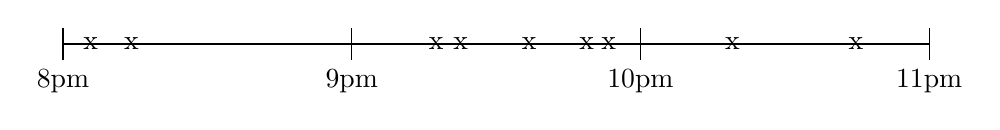
\begin{tikzpicture}

\draw (0,0) -- (11,0)
  node[pos=0.35/11]{x}
  node[pos=0.87/11]{x}
  node[pos=4.74/11]{x}
  node[pos=5.05/11]{x}
  node[pos=5.92/11]{x}
  node[pos=6.65/11]{x}
  node[pos=6.93/11]{x}
  node[pos=8.50/11]{x}
  node[pos=10.07/11]{x}
;
\node[below] at (0,-.2) {8pm};
\draw (0,-.2) -- (0,.2);
\node[below] at (11/3,-.2) {9pm};
\draw (11/3,-.2) -- (11/3,.2);
\node[below] at (22/3,-.2) {10pm};
\draw (22/3,-.2) -- (22/3,.2);
\node[below] at (11,-.2) {11pm};
\draw (11,-.2) -- (11,.2);


\end{tikzpicture}
\end{center}

Let the random variable $Y$ be the number of tweets from
the celebrity in some time interval.
When we say that the number of tweets in a time interval $t$ follows
a Poisson distribution with mean $\lambda t$, we write
\[
  Y \sim \text{Poisson($\lambda t$)}
\]
If $t$ is one hour, then we can write
\[
  Y \sim \text{Poisson($\lambda = 3$)}
\]
Stating that the number of tweets follows a Poisson distribution
implies that the time between tweets follows an Exponential
distribution (and vice versa). Let the random variable $X$ be
the time between tweets. Then
\[
  Y \sim \text{Poisson($\lambda t$)} \Longleftrightarrow X \sim \text{Exp($\lambda$)}
\]
Yes, it is the same $\lambda$ in each distribution.
The average number of tweets is $\lambda=3$ per hour. The average
time between tweets is $1/\lambda = 1/3$ hour (or 20 minutes).
Recall that for the Exponential distribution
\[
  E(X) = \frac{1}{\lambda} = \frac{1~\text{hour}}{3~\text{tweets}} = 20 ~\text{minutes per tweet on average}
\]

Questions.
\begin{enumerate}
\item What is the probability that the celebrity sends out five or
  more tweets in one hour?
\item What is the probability that the celebrity sends out
  no tweets between 9pm and 11pm?
\end{enumerate}

\section{Queueing Models}

\section{Exercises}

\begin{enumerate}
  
\subsubsection*{Modeling with Probability Distributions.}

% this problem is OK
% Geometric
\item \emph{Searching for an item.} Albert has \num{1176} Pok\'{e}mon
  cards in total.  Pok\'{e}mon EX is a special type of card, and
  Albert has 39 EX-type cards.  He is looking for an EX-type card, but
  all of the cards are completely mixed up and stored in a shoe
  box. His mother is calling him for dinner.  What is the probability
  that Albert will have to look through no more than 25 cards before
  he finds an EX-type card?

\begin{solution}
\bs Consider finding an EX-type card to be a ``success''. Let $X$ be a
random variable that represents the number of cards that Albert has to
handle up to and including the first success. Then
\[
X \sim \text{Geometric}(p=\frac{39}{1176})
\]
and
\[
P(X \leq 25) = 1 - (1 - p)^{25} \approx 0.57.
\]
\end{solution}

% this problem is OK
% Binomial, odds, probabilities
\item \emph{Playing Pok\`{e}mon.} Albert is playing
  Pok\'{e}mon cards with his friend. It's Albert's turn, and he
  decides to use Marowak. The card says the following.
\begin{quote}
\emph{Flip a coin four times. The amount of damage done to your opponent's
Pok\'{e}mon is the number of heads times 40.}
\end{quote}
What are the odds that Marowak will do at least 120 damage to the
opponent? One approach to answer this question is to use the Binomial
distribution to compute the probability of doing at least 120 damage
and then convert from probability to odds. You can take another
approach if you prefer. In any case, assume that the coin is fair,
i.e.\ the probability of getting heads on any particular toss is 1/2.

\begin{solution}
\bs
In order to do at least 120 damage, we need either three or four heads
out of the four coin tosses. Let $X$ represent the number of heads obtained
in four tosses of a fair coin. Then $X \sim \text{Binomial}(p=1/2,n=4)$.
\begin{align*}
P(X=3) + P(X=4) &= {4 \choose 3} p^3 (1-p)^1 + {4 \choose 4} p^4 (1-p)^0 \\
&= \frac{1}{4} + \frac{1}{16} \\
&= \frac{5}{16}
\end{align*}
The odds are
\[
\frac{p}{1-p} = \frac{\frac{5}{16}}{1-\frac{5}{16}} = \frac{5}{11}
\]
or 5 to 11.
\end{solution}

% this problem is OK
% Exponential distribution
\item \emph{Evaluating a warranty.}
  A manufacturer of automotive batteries offers a one-year
  warranty. If the battery fails for any reason during the warranty
  period, it is replaced for free. The time to failure is distributed
  Exponential with rate $\lambda=.125$ failures per year.
\begin{enumerate}
\item What proportion of batteries fail within the warranty period?
\item The cost to manufacture a battery is \$50, and the profit
per battery is \$25. What is the effect of the warranty replacement
policy on profit? \label{ex:profit}
\end{enumerate}

\begin{solution}
  \bs The question is asking for the theoretical proportion of
  batteries that fail within one year. Since all batteries have the
  same probability of failure, this proportion is equal to the
  probability that a single battery will fail within one year. Let $X$
  be a random variable that represents the time to failure.
\[ P(X<1) = 1-e^{-\lambda t} = 1 - e^{-.125} = 0.118 \]
Now, imagine that the manufacturer has, over time,
  sold many batteries and has kept data on how many batteries failed
  within one year. The empirical proportion is simply the number
  of batteries that failed divided by the number of batteries sold.
  The Law of Large Numbers tells us that when the number of batteries
  sold is large, the empirical proportion will be approximately
  equal to the theoretical proportion.

Taking the warranty into account, the average profit per battery is
\[ \$25 - 0.118\times \$50 = \$19.10 \]
So, the (average) effect of the warranty on profit is -\$5.90.
\end{solution}

% this problem has been re-written
% Poisson distribution
\item \emph{Donut giveaway.}  A professional baseball team has just
  won a game that secured them a berth in the league’s playoffs. To
  celebrate, a local donut shop will be giving away up to 200 free
  donuts during a two-hour period on the morning following the
  victory. All 200 donuts will be baked and decorated with a baseball
  theme before the giveaway starts. If there are any donuts remaining
  after the giveaway, they will be sold at a discounted price. Assume
  that customers will arrive at the giveaway according to a Poisson
  process at a mean rate of 100 customers per hour. Also, note that
  there is a limit of one donut per customer.
\begin{enumerate}
	\item What is the probability that there will be donuts remaining after the giveaway? \label{ex:donuta}
	\item What is the predicted number of donuts that will be remaining after the giveaway? \label{ex:donutb}
\end{enumerate}

For part~\ref{ex:donuta}, present your answer as an expression for the
probability that there will be donuts remaining. Then, use software,
such as R, to compute a numerical answer.

\begin{solution}
  \bs Given that customers arrive to the giveaway according to a
  Poisson process with a mean of 100 customers per hour, the number of
  customers that arrive during the two-hour period is Poisson
  distributed with a mean of 200. Let $N$ be the number of customers
  arriving in a two-hour period. Then
\[ N ~ \text{Poisson}(\lambda = 200) \]
For part~\ref{ex:donuta}, the probability that there will be donuts remaining after the giveaway is 
\begin{align*}
      P(N < 200) &= \sum_{n=0}^{199} \frac{\lambda^n e^{-\lambda}}{n!}\\
      &= \sum_{n=0}^{199} \frac{200^n e^{-200}}{n!}\\
      &\approx .49
\end{align*}
In R,
\begin{Verbatim}
> sum(dpois(0:199,200))
[1] 0.4905966
\end{Verbatim}  

For part~\ref{ex:donutb}, our calculations are all done in expectation
(that is to say, on average). There are 200 customers in 2 hours,
which means that 200 donuts are given away. So, on average, no donuts
are remaining.
\end{solution}

% re-written by hannah
% Poisson distribution
\item \emph{Startup expenses.}  Two friends are starting a small
  business selling ice cream. They applied for a grant and have
  received \$\num{1800} to help cover any startup expenses. The
  friends will incur expenses of \$300 randomly throughout the first
  year, and the time between payments for these expenses is
  exponential with a mean of 2 months. Determine the probability that
  the friends will run out of grant money before the end of the year.

\begin{solution}
  \bs Let $X$ be a random variable that represents the time between
  payments. The mean time between payments, that is to say the
  expected value of $X$ ($E(X)$), is two months. We know that for the
  Exponential distribution
  \[ E(X) = \frac{1}{\lambda} \] where $\lambda$ is the rate (in units
  of payments per month). So,
  \[ X \sim \text{Exp}(\lambda = 1/2~\text{payments per month}) \] If
  the time between payments is distributed Exponential with rate
  $\lambda$, then the number of payments in $t$ months is Poisson with
  mean $\lambda t$. Let $N$ be the number of payments in 12 months.
  \[ N \sim \text{Poisson}(\lambda t = \lambda \times 12 = 6) \] Now,
  the probability that the friends runs out of money is
\begin{align*}
      P(N \geq 6) &= 1 - P(N \leq 5) \\
      &= 1 - \sum_{n=0}^{5} \frac{\lambda^n e^{-\lambda}}{n!}\\
      &= 0.55
\end{align*}
You may have defined the event that the friends runs out of
money as $P(N = 6)$. In other words, that there are exactly
six payments during the first year.  This is incorrect because
we are modeling the spending activity as a Poisson process. In
other words, the (unstated) assumption is that the number of
payments is independent of the available funds.
\end{solution}

% this problem needs to be re-written, but it can be very similar.
% Poisson distribution
\item \emph{Stocking a vending machine.}
A university cafeteria has a vending machine that is stocked with a variety of juices and sodas. A vending machine attendant replenishes inventory weekly so that there are 180 beverages in stock at the beginning of each week. The cafeteria is open 24 hours, 7 days a week, and it is expected that the beverages will be purchased according to a Poisson distribution with a mean of 1 hour between purchases.
\begin{enumerate}
	\item What is the probability that there are no beverages remaining in the vending machine when the attendant arrives? \label{ex:pout}
	\item On average, how many beverages will be remaining in the vending machine when the attendant arrives? \label{ex:qremain}
	\item What is the probability that the attendant will replenish 150 or more beverages? \label{ex:preplenish}
\end{enumerate}

\begin{solution}
	\bs
	For part~\ref{ex:pout}, there will be no beverages remaining in the vending machine if 180 or more beverages are purchased before the end of the week. Because the beverages are purchased according to a Poisson distribution with a mean of one hour between purchases, the rate $\lambda$ that beverages are purchased is 24 beverages per day. Therefore, the number of purchases in 7 days is Poisson with mean $\lambda t$. Let $N$ be the number of purchases in 7 days.
	\[ N \sim \text{Poisson}(\lambda = \lambda \times 7 = 168) \]
	Let
	$D$ be a random variable that represents demand for beverages during one week.
	\begin{align*}
		P(D \geq 180) &= 1 - P(D \leq 179)\\
		&= 1 - \sum_{n=0}^{179} \frac{168^n e^{-168}}{n!}\\
		&\approx 0.19
	\end{align*}
	In R,
	\begin{Verbatim}
	> 1 - sum(dpois(0:179,168))
	[1] 0.1866995
	\end{Verbatim}
	
	For part~\ref{ex:qremain}, the expected number of purchases from the vending machine each week is 168 beverages. Therefore, the expected number of beverages remaining at the end of the week is $180-168=12$ beverages.
	
	For part~\ref{ex:preplenish}, 150 or more beverages will be replenished if 150 or more beverages are purchased before the end of the week. The probability that 150 or more beverages are purchased during a week is 
	\begin{align*}
		P(D \geq 150) &= 1 - P(D \leq 149)\\
		&= 1 - \sum_{n=0}^{149} \frac{168^n e^{-168}}{n!}\\
		&\approx 0.93
	\end{align*}
	In R,
	\begin{Verbatim}
	> 1 - sum(dpois(0:149,168))
	[1] 0.9253016
	\end{Verbatim}
\end{solution}

% this problem needs to be re-written.
% Poisson distribution
\item \emph{Making cookies.} A baker blends 800 chocolate chips into a
  dough mix and, from this, makes 500 cookies.
\begin{enumerate}
\item Find the probability that a randomly picked cookie will have 
exactly three chocolate chips. \label{a}
\item Find the probability that a randomly picked cookie will have
  at least two chocolate chips. \label{b}
\end{enumerate}
Assume that the chocolate chips are mixed thoroughly,
and in a random fashion. Let $X$ be a random variable that represents
the number of chips in a cookie, and assume that $X$ follows a 
Poisson distribution.

\begin{solution}
\bs For part~\ref{a}, we want to know $P(X=3)$.  With 800 chips
randomly mixed into 500 cookies, there will be, on average, $800/500 =
1.6$ chips per cookie.  Then $X \sim \text{Poisson}(\lambda = 1.6)$.
\[
P(X=3) = \frac{e^{-\lambda}\lambda^3}{3!} = \frac{e^{-1.6}1.6^3}{6} = 0.138
\]
For part~\ref{b}, the probability that a cookie has at least two
chips is
\begin{align*}
P(X \geq 2) = 1 - P(X \leq 1) &= 1 - P(X=0) - P(X=1) \\
&= 1 - \frac{e^{-1.6}\times 1.6^0}{0!} - \frac{e^{-1.6}\times 1.6^1}{1!} \\
&= 0.475
\end{align*}
\end{solution}

% this problem is OK
% a poisson process, memory-less property of exponential distribution
\item A dump truck at a mine takes ore to the railroad after 10
  one-ton scoops have been loaded into the truck.  The one-ton scoops
  are loaded from a large diesel-powered shovel independently and at a
  mean rate of seven scoops per hour.  The time between scoops from the
  shovel can be considered to follow an Exponential distribution.

\begin{enumerate}
\item Find the probability that the time between consecutive trips to
  the railroad will be at least one hour.
\item It takes the dump truck 18 minutes to travel to the railroad,
  unload, and return. Suppose the truck returns and finds that no
  scoop is ready to be loaded. What is the probability that the next
  scoop is ready within 5 minutes? \label{item:2}
\end{enumerate}

\begin{solution}
  \bs The time between scoop arrivals is distributed Exponential, so
  we know that the number of arrivals in a time interval is
  distributed Poisson. In particular, the number of arrivals in a
  one-hour period follows a Poisson distribution with mean
  $\lambda=7$. In order for the time between consecutive trips to the
  railroad to take at least one hour, we require that the number of
  arrivals in one hour is nine or less. Let $X$ be the number of
  (scoop) arrivals in a one hour period.
\[
P(X \leq 9) = \sum_{x=0}^9 \frac{e^{-\lambda}\lambda^x}{x!} = .83.
\]
For part \ref{item:2}, we can invoke the memoryless property of the
Exponential distribution. The remaining time until the next arrival is
disitributed Exponential with rate 7 scoops per hour, regardless of how
much time has elapsed since the last arrival. Let $Y$ be the time
until the next arrival, and don't forget to convert from minutes to
hours.
\[
P(Y \leq 5) = 1 - e^{-7\times \frac{5}{60}} = .44
\]
\end{solution}

% this problem needs to be re-written
% normal distribution
\item Normal distribution. A final exam is constructed so that the
  test scores $x$ are approximately normally distributed, with
  parameters $\mu$ and $\sigma$. The instructor (who is nicer than me)
  assigns letter grades to the test scores as shown in the table
  below. This is known as ``grading on the curve''. What fraction of
  the class gets A, B, C, D, F?

\begin{tabular}{lc}
test score & letter grade \\ \hline
$\mu+\sigma < x$ & A \\
$\mu < x < \mu+\sigma$ & B \\
$\mu-\sigma < x < \mu$ & C \\
$\mu-2\sigma < x < \mu-\sigma$ & D \\
$x < \mu-2\sigma$ & F
\end{tabular}

\vspace{.1in}
\begin{solution}
\bs
\begin{align*}
\text{A}&\quad 1-P(X<\mu+\sigma)=1-\Phi(1) = .159 \\
\text{B}&\quad P(X<\mu+\sigma)-P(X<\mu)=\Phi(1)-\Phi(0) = .341 \\
\text{C}&\quad P(X<\mu)-P(X<\mu-\sigma)=\Phi(0)-\Phi(-1)=.341 \\
\text{D}&\quad P(X<\mu-\sigma)-P(X<\mu-2\sigma)=\Phi(-1)-\Phi(-2)=.136 \\
\text{F}&\quad P(X<\mu-2\sigma)=\Phi(-2) = .023
\end{align*}
\end{solution}

% this problem needs to be re-written
% Lognormal distribution
\item \emph{Stock prices.} The prices of stocks are often modeled
  with a lognormal distribution. An investor is considering purchasing
  stock in one of two companies, A or B. The price of a share of stock
  today is \$1 for both companies. For company A, the value of the
  stock one year from now is modeled as lognormal with parameters
  $\mu=.05$ and $\sigma=.1$. For company B, the value of the stock one
  year from now is modeled as lognormal with parameters $\mu=.02$ and
  $\sigma=.2$.
\begin{enumerate}
\item Find the mean of the price of one share of company A one year
  from now. \label{a1}
\item Find the probability that the price of one share of company A
  one year from now will be greater than \$1.20. \label{a2}
\item Find the mean of the price of one share of company B one year
  from now. \label{b1}
\item Find the probability that the price of one share of company B
  one year from now will be greater than \$1.20. \label{b2}
\end{enumerate}

\begin{solution}
\bs Let $X_A$ and $X_B$ be the price of one share of company A and
company B one year from now, respectively. We know from the problem
description that $X_A \sim \text{LogN}(\mu=.05,\sigma=.1)$ and $X_B
\sim \text{LogN}(\mu=.02,\sigma=.2)$.

For part~\ref{a1}, the mean of $X_A$ is
\[
e^{\mu + \sigma^2/2} = \$1.06
\]
For part~\ref{a2}, 
\begin{align*}
P(X_A > \$1.20) &= P(\ln(X_A) > \ln(1.20)) \\
&= P\left(Z > \frac{\ln(1.20)-.05}{.1}\right) \\
&= P(Z > 1.323) \\
&= 1-P(Z < 1.323) \\
&= .093
\end{align*}
For part~\ref{b1}, the mean of $X_B$ is
\[
e^{\mu + \sigma^2/2} = \$1.04
\]
For part~\ref{b2}, 
\begin{align*}
P(X_B > \$1.20) &= P(\ln(X_B) > \ln(1.20)) \\
&= P\left(Z > \frac{\ln(1.20)-.02}{.2}\right) \\
&= P(Z > .812) \\
&= 1-P(Z < .812) \\
&= .208
\end{align*}
\end{solution}

\subsubsection*{Stochastic Processes}

\subsubsection*{Queueing Models}

% this problem is ok.
\item \emph{Performance metrics for a queueing system.} Consider a
  single server queueing system with FIFO queue discipline.  For the
  particular day that this system was in operation, the arrival times
  and the service times of the first six customers were
  (0,3,7,9,10,12) and (4,6,2,1,3,1), respectively. Arrival times and
  service times are in minutes.  Compute the average waiting time and
  the average number of customers in the queue for the first six
  customers. It will help to construct a diagram of number in
  system versus time.

\begin{solution}
\bs
    
\pgfplotsset{compat=1.12}
\begin{center}
  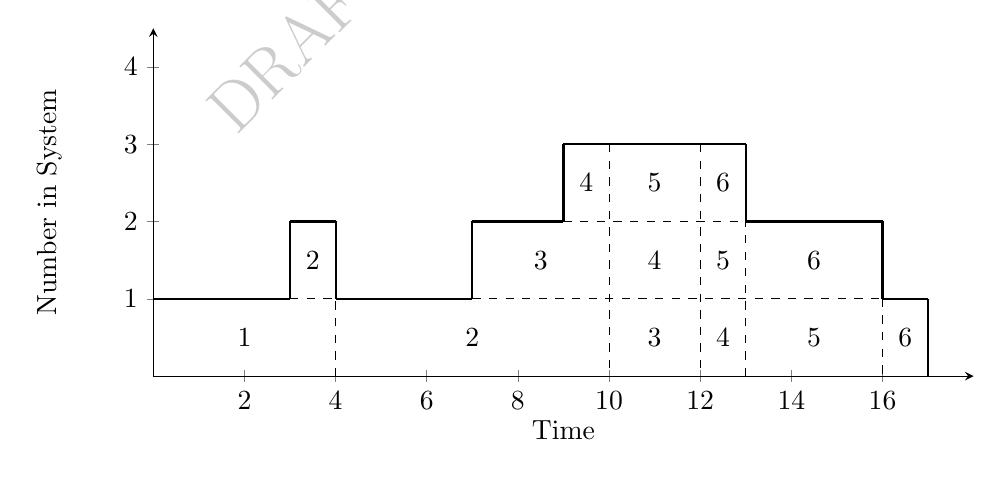
\begin{tikzpicture}[scale=1.0]
    \begin{axis}[clip=false,
      width=12cm, height=6cm,
    axis x line=middle,
    axis y line=middle,
    ymin=0, ymax=4.5,
    ytick={0,1,2,3,4},
    yticklabels={0,1,2,3,4},
    xmin=0, xmax=18,
    xtick={2,4,6,8,10,12,14,16},
    xticklabels={2,4,6,8,10,12,14,16},
    x label style={at={(axis description cs:0.5,-0.1)},anchor=north},
    y label style={at={(axis description cs:-0.1,.5)},rotate=90,anchor=south},
    xlabel=Time,
    ylabel=Number in System,
    ]
    \addplot[mark=none, style=thick] coordinates { (0, 1) (3, 1) };
    \addplot[mark=none, style=thick] coordinates { (3, 1) (3, 2) };
    \addplot[mark=none, style=thick] coordinates { (3, 2) (4, 2) };
    \addplot[mark=none, style=thick] coordinates { (4, 1) (4, 2) };
    \addplot[mark=none, style=thick] coordinates { (4, 1) (7, 1) };
    \addplot[mark=none, style=thick] coordinates { (7, 1) (7, 2) };
    \addplot[mark=none, style=thick] coordinates { (7, 2) (9, 2) };
    \addplot[mark=none, style=thick] coordinates { (9, 2) (9, 3) };
    \addplot[mark=none, style=thick] coordinates { (9, 3) (13,3) };
    \addplot[mark=none, style=thick] coordinates { (13, 3) (13,2) };
    \addplot[mark=none, style=thick] coordinates { (13,2) (16,2) };
    \addplot[mark=none, style=thick] coordinates { (16,2) (16,1) };
    \addplot[mark=none, style=thick] coordinates { (16,1) (17,1) };
    \addplot[mark=none, style=thick] coordinates { (17,1) (17,0) };

    \addplot[mark=none,dashed] coordinates { (3,1) (4,1) };
    \addplot[mark=none,dashed] coordinates { (7,1) (16,1) };
    \addplot[mark=none,dashed] coordinates { (9,2) (13,2) };
    \addplot[mark=none,dashed] coordinates { (10,3) (10,0) };
    \addplot[mark=none,dashed] coordinates { (12,3) (12,0) };
    \addplot[mark=none,dashed] coordinates { (16,1) (16,0) };
    \addplot[mark=none,dashed] coordinates { (4,0) (4,1) };
    \addplot[mark=none,dashed] coordinates { (13,0) (13,2) };

    \node at (2,.5) {1};
    \node at (3.5,1.5) {2};
    \node at (8.5,1.5) {3};
    \node at (9.5,2.5) {4};
    \node at (7,.5) {2};
    \node at (11,.5) {3};
    \node at (11,1.5) {4};
    \node at (11,2.5) {5};
    \node at (12.5,.5) {4};
    \node at (12.5,1.5) {5};
    \node at (12.5,2.5) {6};
    \node at (16.5,.5) {6};
    \node at (14.5,.5) {5};
    \node at (14.5,1.5) {6};

  \end{axis}
\end{tikzpicture}
\end{center}

First note that the problem description does \emph{not} tell us that
the times between arrivals and/or the service times are exponentially
distributed. So it is not an $M/M/1$ system.
The total delay of all six customers is $0+1+3+3+3+4=14$. The average
waiting time in the queue is the total delay divided by the number
of customers.
\[ W_q = \frac{14}{6} = 2.3333~\text{min} \]
To compute the average number in the queue, weight the time in queue
by the number of customers. In other words, compute the area under the
curve but above one, and then divide by the total time.
\[ L_q = \frac{14}{17} \]

\end{solution}

% this problem needs to be re-written.
\item \emph{Justification for a capital expense.}
  Cars arrive at the Lincoln Tunnel toll gate according to a Poisson
  process with an average rate of 90 cars per hour. The time for passing
  the gate is exponential with mean 38 seconds.  Drivers complain of
  the long waiting time, and authorities are willing to reduce the
  average passing time to 30 seconds by installing automatic toll
  collecting devices, provided two conditions are satisfied: 1) the
  average number of waiting cars in the present system exceeds 5 and
  2) the percentage of the gate idle time with the new device
  installed does not exceed 10\%. Can the new device be justified?

\begin{solution}
\bs
Cars arrive at the rate
\[ \lambda = 90~\text{cars per hour} \times 1/3600 =
  1~\text{car}/40~\text{seconds} \]
We know that $\mu=1/38$
for the current system and $\mu_{\text{new}}=1/30$ for the new
system.
Condition 1 states that the average number of waiting
cars in the current system must exceed 5.
\[ L_s = \frac{\lambda}{\mu-\lambda} = \frac{1/40}{1/38-1/40} = 19 \]
You may have also computed
\[ L_q = \frac{\lambda^2}{\mu(\mu-\lambda)} =
  \frac{(1/40)^2}{(1/38)(1/38 - 1/40)} = 18.05 \]
Either way, the first condition is satisfied. The second condition
states that the percentage of idle time in the new system cannot
exceed 10\%.
\[ p_0 = 1 - \frac{\lambda}{\mu_{\text{new}}} = 1 - \frac{1/40}{1/30} = .25 \]
The second condition is not satisfied. There is no justification
for the new toll gate device.
\end{solution}

% this problem needs to be re-written
\item \emph{Comparing system configurations.}
  Pete's Market is a small local grocery store with one checkout counter.
  Shoppers arrive at the checkout lane according to a Poisson process,
  with an arrival rate of 15 customers per hour. The checkout service times
  are distributed Exponential with a service rate of 20 customers per hour.
  The manager is considering two options for improving service.
  \begin{compactenum}
    \item Hire a second person to bag groceries while the cashier is scanning
      and collecting money from the customer. With this improved single-server
      operation, the service rate would be increased to 30 customers per hour.
    \item Hire a second person to operate a second checkout counter. The
      two-server operation would have a service rate of 20 customers per
      hour for each server.
  \end{compactenum}
  Determine the improvements that would result, consider the
  relative cost of each option, and make a recommendation to the manager.

\begin{solution}
\bs Let's look at the average number in the queue $L_Q$ and the
average time in queue $W_Q$ as metrics to judge improvement in
system performance. Because the interarrival times and the service
times are exponentially distributed, we can use the results from
section 11.2. Before any improvements are made,
\[ L_q = \frac{\lambda^2}{\mu(\mu-\lambda)} = \frac{15^2}{20(20-15)} = 2.25~\text{cust} \]
and
\[W_q = \frac{L_q}{\lambda} = \frac{2.25}{15} = .15~\text{hour} = 9~\text{min} \]
If they add a second person to the existing single checkout
\[ L_q = \frac{\lambda^2}{\mu(\mu-\lambda)} = \frac{15^2}{30(30-15)} = 0.5~\text{cust} \]
and
\[W_q = \frac{L_q}{\lambda} = \frac{0.5}{15} = 0.0333~\text{hour} = 2~\text{min} \]
and if they add a completely separate second checkout then we
need to use the formulas from section 11.3 for a two-server operation. First,
\[ P_0 = \frac{1}{\sum_{n=0}^{k-1}\frac{\left(\lambda/\mu\right)^n}{n!} + \frac{\left(\lambda/\mu\right)^k}{k!}\left(\frac{k\mu}{k\mu-\lambda}\right)} \]
where $k=2$ servers. Then
\[ L_q = \frac{\left(\lambda/\mu\right)^k\lambda\mu}{(k-1)!(k\mu-\lambda)^2}P_0 \]
and
\[W_q = \frac{L_q}{\lambda}  \]
Plugging values, I got $P_0=0.4545$, $L_q=0.123$, and $W_q=0.0082$ hours or 0.5 minutes.
Considering the relative improvement and the cost
of adding a second checkout, I would recommend option a). That is, to
add a second person to the existing checkout. The average number in
queue and the average time in queue appear to be acceptable for a
grocery store.
\end{solution}


\end{enumerate}

\chapter{Decision Problems}

\section{Games Against Nature}

\section{Games Against an Opponent}

% this will be the last portion of this section, where we bring together
% several concepts. Need to re-write this section: change the context
% of the problem and explain the methodology.
\emph{Nature as an adversary: a two-person zero-sum game.}
Merrill has a concession stand at Target Field for the sale of
sunglasses and umbrellas. This entrepreneur likes to make sales
regardless of the weather.  When it rains can sell about 500
umbrellas.  On a sunny day he can sell about 100 umbrellas and about
1000 sunglasses. Umbrellas cost him 50 cents and sell for \$1.
Sunglasses cost him 20 cents each and sell for 50 cents. Merrill is
willing to invest \$250 in the concession stand business.  All unsold
items represent a loss; there is no salvage value. 

Formulate Merrill's problem as a two-person zero--sum game. Merrill is
the row player and Nature is the column player. Merrill's strategy set
is \{buy inventory for rain, buy inventory for sun\}. Nature's strategy
set is \{rain, sun\}. The payoff entries represent the profit/loss.
Find an equilibrium strategy for Merrill. That is
to say, Merrill treats Nature as a strategic opponent and wants to
find an optimal inventory strategy that will yield a maximum expected
profit \emph{regardless} of the weather.

Would Merrill necessarily need to invest all \$250 into buying inventory
exclusively for rain or sun? In other words, does it seem possible that
Merrill could truly mix his two pure strategies and invest a portion
of the \$250 into each? The game is

\begingroup
\setlength{\tabcolsep}{9pt}
\renewcommand*{\arraystretch}{2}
\begin{tabularx}{4in}{YYYY}
& & \multicolumn{2}{c}{Nature} \\
& & Rain & Sun \\ \cline{3-4}
\multirow{2}{.5in}{Merrill} & \gtcol{Rain} & \gtcol{250} & \gtcol{-150} \\ \cline{3-4}
& \gtcol{Sun} & \gtcol{-150} & \gtcol{350} \\ \cline{3-4}
\end{tabularx}
\endgroup
\vspace{.1in}

The best strategy for Merrill is to mix buying for rain and buying
for sun in the ratio 5 to 4. These are the odds. To compute 
Merrill's expected profit (i.e. the value of the game) we use
Merrill's  equilibrium strategy against either of Nature's
pure strategies. Here is the payoff for Merrill against
Nature's strategy of Rain.

\[ \frac{5 \times (250) + 4 \times (-150)}{9} = \$72.22 \]

Merrill could play the odds and choose a pure strategy, but 
note that in this game it is possible for Merrill to physically
mix the strategies. He could invest 5/9 of his \$250 in
rainy--day inventory and invest 4/9 in sunny--day inventory.
So he buys
\[ \frac{5}{9} \left(500 \times .50\right) + \frac{4}{9} \left(100 \times .50\right) = \$161.11 \]
worth of umbrellas and
\[ \frac{4}{9} \left(1000 \times .20\right) = \$88.89 \]
worth of sunglasses so that he enjoys a steady profit of \$72.22.

\section{Exercises}
\begin{enumerate}
	
% This exercise is OK
\item \emph{Rules for decision--making under ignorance.}
  You have the opportunity to go on a
  blind date, but you are hesitant.  You are lonely and would like to
  find the love of your life; however, you dislike awkward
  situations. Furthermore, you find it difficult to estimate the
  probability that this particular blind date will turn out to be the
  love of your life, but you know this probability is
  non-negligible. To be a little more precise, you have the following
  values: finding the love of your life is worth 1000, being in an
  awkward date situation (i.e. being on a date and knowing that you
  will not see the person again) is worth -10, and staying home
  watching Netflix is worth zero.

\begin{enumerate}
\item Formulate a decision problem for deciding whether to go on the
blind date or to stay home.
\item Use the maximin rule to solve the problem.
\item Use the minimax regret rule to solve the problem.
\end{enumerate}

\begin{solution}
\bs The decision problem can be represented with the following table.
\\[.1in]
\begin{tabular}{ccc}
 \multicolumn{3}{c}{decision matrix} \\
 & find love & lots of awkward moments \\ \cline{2-3}
go on date & 1000 & -10 \\
decline date & 0 & 0 
\end{tabular}
\\[.1in] 
The maximin rule tells you to decline the date because it has
the best of all the worst possible outcomes. To use minimax regret, we
form the regret matrix.  \\[.1in]
\begin{tabular}{ccc}
 \multicolumn{3}{c}{regret matrix} \\
 & find love & lots of awkward moments \\ \cline{2-3}
go on date & 0 & -10 \\
decline date & -1000 & 0
\end{tabular}
\\[.1in] Minimax regret tells you to go on the date because the
possibility of not finding love has the most regret.
\end{solution}

% written by Emily
\item \emph{Gardening against nature.} A family is considering growing
  their own garden to save money on fresh vegetables. They have space
  in their yard for the garden but would need to purchase seeds and
  gardening supplies. The family is excited to grow a garden, but they
  know there are a lot of hungry rabbits in their neighborhood that
  might eat their plants before the family can harvest any vegetables
  from them. Money saved by the garden is shown in the following
  table.

\begin{tabular}{rcc}
& \multicolumn{2}{c}{State of Nature} \\
& $s_1$ & $s_2$ \\
& rabbits leave garden alone & rabbits eat garden \\ \cline{2-3}
plant garden & \$400 & -\$100\\
buy vegetables from store & 0 & 0
\end{tabular}

\begin{enumerate}
    \item If the probability that the rabbits leave the garden alone is 0.3, what decision is recommended for the family? What are the expected savings?
    
    \item The family has the option to purchase fast-growing plant seeds (the fast-growing seeds are the same price as regular seeds but they must buy the fast-growing seeds now if they want them because they are in high demand).  With these fast-growing seeds, the family can wait three more weeks to plant their garden. During that time, some scientists will finish their study on the appetites of the local rabbits, and the family will have a better idea about the probability that their garden is eaten by rabbits. They can return the seeds later for a partial refund if they do not use them.
    Let $L$ represent the event the rabbits have large appetites and let $S$ represent
    the event that rabbits have small appetites. Then
    \[
    \begin{matrix}
    P(L)=0.60, & P(s_1 \mid L)=0.15, & P(s_2 \mid L)=0.85,\\
    P(S)=0.40, & P(s_1 \mid S)=0.79, & P(s_2 \mid S)=0.21.
    \end{matrix}
    \]
    What is the optimal decision strategy if the family purchases the fast-growing seeds so they can wait and learn more about the rabbit appetites before making a decision?
    
    \item If \$40\ of the fast-growing seed purchase is non-refundable, should the family purchase the fast-growing seeds? Why or why not? What is the maximum non-refundable amount the family should pay to get the fast-growing seeds?
\end{enumerate}

\begin{solution}
\bs For part a), the expected savings when planting the garden are
\[ 400 \times 0.3  - 100 \times 0.7 = \$50. \]
The savings from not planting the garden are \$0, so based on expected value,
the best decision is to plant the garden.

For part b), if the rabbits have large appetites ($L$), then planting 
the garden would result in -\$25 of expected savings.
If the rabbits have small appetites ($S$), then planting the garden will result in \$295 
of expected savings. 

If L, \[ \$100 \times 0.15 - \$100 \times 0.85 = -\$25 \]
If S, \[ \$400 \times 0.79 - \$100 \times 0.21 = \$295 \]

Not planting will always result in \$0 of savings. 
The optimal decision strategy is to plant the garden if $S$ and buy vegetables 
from the store if $L$.

For part c), we use the optimal decision for each possible event $L$ and $S$. 
The expected savings from purchasing the fast-growing seeds
(but before actually purchasing the seeds) are
\[ \$0 \times 0.60 + \$295 \times 0.40 = \$118 \]
The maximum non-refundable amount that the family should be willing 
to pay for the fast-growing seeds is
\[ \$118 - \$50 = \$68 \]
\end{solution}

% this problem is OK
\item \emph{Using Baye's formula to update a prior belief.}
Curling is a sport in which players slide a stone over ice toward a
target. The association governing the sport has implemented drug
testing. It is believed that 15\% of all curlers use banned drugs to
enhance performance. If a player uses banned drugs, the association
may take away any prizes that the player has won; however, it
undesirable to falsely accuse someone of using banned substances.  The
utilities for each decision and state of nature are

\begin{center}
\begin{tabular}{rrrr}
& drug use & no drug use \\ \cline{2-3}
take away prizes & -100 & -1000 \\
do not & -600 & 0 
\end{tabular}
\end{center}

Notice that there is a small dis-utility for taking prizes away from a drug user
due to bad publicity for the sport. The test to detect drug use is
less than 100\% reliable. In particular, if $D$ indicates that a 
player uses banned drugs, and $+$/$-$ indicate a positive/negative
test result, then the true positive rate and the true negative rate
are
\[
P(+ \mid D) = .97 \quad \text{and} \quad P(- \mid \overline{D}) = .97,
\]
respectively, Given the utilities and the accuracy of the test, what is the best
decision if a player has a positive test result? (The association
wants to maximize expected utility.)

\begin{solution}
\bs First we update the probability of drug use via Baye's formula.
\begin{align*}
P(D \mid +) &= \frac{P(D \cap +)}{P(+)} \\
&= \frac{P(+ \mid D)P(D)}{P(+ \mid D)P(D) + P(+ \mid \overline{D})P(\overline{D})} \\
&= \frac{.97 \times .15}{.97 \times .15 + .03 \times .85} \\
&= .851
\end{align*}
and then we can compute $P(\overline{D} \mid +) = 1 - P(D \mid +) = .149$.
Using these posterior probabilities, the expected utilities are
\begin{align*}
E(\text{take away}) &= (-100)(.851) + (-1000)(.149) = -234 \\
E(\text{do not}) &= (-600)(.851) = -511
\end{align*}
The best decision is to take away prizes when a player tests positive.
\end{solution}

% Emily - expected value and sensitivity analysis
\item \emph {Decisions under risk and sensitivity analysis.}  The
  owners of a popular outdoor furniture company predict that their
  sales will double this coming year. The company is already producing
  the maximum amount of furniture possible in their current
  facility. They are considering expanding their manufacturing
  facility to accommodate the predicted increase in demand. If
  undertaken, the expansion will cost \$\num{500000}. If the demand
  doubles as predicted, revenue will increase by \$\num{800000}.  If
  the predicted increase in demand proves to be too optimistic,
  revenue will increase by only \$\num{250000}.  If the expansion is
  not undertaken, the company will lose \$\num{50000} due to
  out-of-stock orders from agitated customers.  The change in demand
  will be determined by next year's weather; more outdoor furniture is
  sold when the weather is nice.  There is a 0.55 chance of good
  weather, which will result in a doubling of demand. There is a 0.45
  chance of poor weather, which will result in only a slight increase
  in demand.

\begin{enumerate}
\item Should the manufacturing facility be expanded? The owners make
  decisions based on expected value.
\item How does the decision change with the probability of good/poor
  weather? To answer this question, you should perform a sensitivity
  analysis.
\end{enumerate}

\begin{solution}
\bs The decision table for this problem is
\begin{center}
\begin{tabular}{rrr}
      & $0.55$ & $0.45$ \\
      & good weather & poor weather \\ \hline
      expansion & \$\num{300000} & -\$\num{250000} \\
      no expansion & -\$\num{50000} & -\$\num{50000}
\end{tabular}
\end{center}

The expected payoff of each decision is
\begin{align*}
&E(\text{expansion}) = 0.55 \times \$\num{300000}
- 0.45 \times \$\num{250000} = \$\num{52500} \\
&E(\text{no expansion}) = -\$\num{50000}
\end{align*}
The company should expand the facility. As the probability of poor
weather increases, the expected value of the expansion
decreases.  Let $p$ represent the probability of poor weather.
\begin{align*}
E(\text{expansion}) &= \num{300000}(1-p) - \num{250000}p \\
&= \num{300000} - \num{550000}p
\end{align*}
The company should expand the facility as long as
\begin{align*}
E(\text{expansion}) &\geq E(\text{no expansion}) \\
\num{300000} - \num{550000}p &\geq -\num{50000} \\
-\num{5500000}p &\geq -\num{350000} \\
p &\leq \frac{7}{11} \approx .64
\end{align*}
Expanding the facility is the best decision unless the probability of
poor weather is greater than .64.
\end{solution}

% written by Emily
\item \emph{Elimination of dominated strategies.}
Two street vendors, A and B, are located near a major tourist attraction. 
The proportion of customers
captured by each vendor depends on the merchandise sold by that vendor and by
her competitor. A customer gained by one is lost to the other. Each vendor
can stock one of the following: clothing, ice cream, or souvenirs.
The possible strategies and proportion of customers captured are as follows.

\begin{tabular}{l}
If both shops sell souvenirs, A captures 75\% of the customers.\\
If both shops sell clothing, A and B split the customers evenly.\\
If both shops sell ice cream, A and B split the customers evenly.\\
If B sells ice cream and A sells souvenirs, A captures 10\%.\\
If B sells clothing and A sells ice cream, A captures 90\%.\\
If B sells souvenirs and A sells clothing, A captures 10\%.\\
If A sells clothing and B sells ice cream, A captures 100\%.\\
If A sells souvenirs and B sells clothing, A captures 75\%.\\
If A sells ice cream and B sells souvenirs, A captures 40\%.
\end{tabular}

\setlength{\parindent}{0cm}
Model the decision of each vendor as two-person zero-sum game
and find a solution by elimination of dominated strategies.

\begin{solution}
\bs The game is

\begingroup
\setlength{\tabcolsep}{9pt}
\renewcommand*{\arraystretch}{2}
\begin{tabularx}{4.5in}{YYYYY}
& & \multicolumn{3}{c}{B} \\
& & clothing & ice cream & souvenirs \\ \cline{3-5}
\multirow{3}{.25in}{A} & \gtcol{clothing} & \gtcol{.50} & \gtcol{1} & \gtcol{.10} \\ \cline{3-5}
& \gtcol{ice cream} & \gtcol{.90} & \gtcol{.50} & \gtcol{.40} \\ \cline{3-5}
& \gtcol{souvenirs} & \gtcol{.75} & \gtcol{.10} & \gtcol{.25} \\ \cline{3-5}
\end{tabularx}
\endgroup
\vspace{.1in}

For A, ice cream strictly dominates souvenirs and for B, souvenirs
strictly dominates clothing, leaving a $2 \times 2$ game.

\begingroup
\setlength{\tabcolsep}{9pt}
\renewcommand*{\arraystretch}{2}
\begin{tabularx}{4in}{YYYY}
& & \multicolumn{2}{c}{B} \\
& & ice cream & souvenirs \\ \cline{3-4}
\multirow{2}{.25in}{A} & \gtcol{clothing} & \gtcol{1} & \gtcol{.10} \\ \cline{3-4}
& \gtcol{ice cream} & \gtcol{.50} & \gtcol{.40} \\ \cline{3-4}
\end{tabularx}
\endgroup
\vspace{.1in}

Now for B, souvenirs dominates ice cream. Then, A will choose to sell
ice cream over clothing. So, the best strategies for A and B are to
sell ice cream and souvenirs, respectively.  Using this pair of
strategies, A will capture 40\% of the customers.
\end{solution}

% written by Emily to replace Goldsen and Kershaw battle of words
\item \emph{A two-person zero-sum game.}  A professional football
  player believes that the team he plays for should be allocating more
  money to the salaries of the players, so he wants his contract to be
  changed to pay him more. His two options are to play in the upcoming
  season or not play in the upcoming season and hope the team will
  negotiate with him. The team knows that he is a valuable player but
  does not want to pay him more or go through the process of
  negotiations. The team has come up with three options to deal with
  the situation: negotiate, refuse to negotiate and play the season
  without him, or increase the player's salary by a set amount with no
  other negotiations. Keep in mind that the player wants to maximize
  his salary, and the team wants to minimize their costs, which means
  keep salaries as low as possible. The utilities/payoffs to
  the player and to the team are described next.

  If the player plays and the team does not negotiate, the player's
  salary will not change.  If the player does not play and the team
  does not negotiate, the player will find a different job as a
  broadcaster for a payoff of 1 because he is such a well-known
  person. This is bad publicity for the team and hurts their jersey
  sales.  If the player plays but the team still negotiates, the
  player will end up with a payoff of 3.  If the player had
  chosen to not play and the team negotiates, the negotiations will go
  poorly and the player will end up with a payoff of -2 for having to
  deal with costs related to poor publicity.  If the team decides
  increase the player's salary with no negotiations, the player will
  end up with a payoff of 2 no matter what he chooses to do.


  Formulate the 2-by-3 game and determine the best strategy for the
  player and for the team.  Who is most likely to come out ahead in
  this situation?
  
\begin{solution}
\bs The game is

\begingroup
\setlength{\tabcolsep}{9pt}
\renewcommand*{\arraystretch}{2}
\begin{tabularx}{4.5in}{YYYYY}
& & \multicolumn{3}{c}{Team} \\
& & negotiate & don't negotiate & increase salary \\ \cline{3-5}
\multirow{2}{.5in}{Player} & \gtcol{play} & \gtcol{3} & \gtcol{0} & \gtcol{2} \\ \cline{3-5}
& \gtcol{don't play} & \gtcol{-2} & \gtcol{1} & \gtcol{2} \\ \cline{3-5}
\end{tabularx}
\endgroup
\vspace{.1in}

The team's strategy of a set
increase is dominated by the strategy to not negotiate, so there is no
reason that they would chose to offer a pre-determined
increase without negotiations. The reduced game is

\begingroup
\setlength{\tabcolsep}{9pt}
\renewcommand*{\arraystretch}{2}
\begin{tabularx}{4in}{YYYY}
      & & \multicolumn{2}{c}{Team} \\
      & & {negotiate} & {don't negotiate} \\ \cline{3-4}
      \multirow{2}{.5in}{Player} & \gtcol{play} & \gtcol{3} & \gtcol{0} \\ \cline{3-4}
      & \gtcol{don't play} & \gtcol{-2} & \gtcol{1} \\ \cline{3-4}
\end{tabularx}
\vspace{.1in}
\endgroup

Since there is no saddle point, the best strategies for the player and
for team are mixed. The player should mix the strategies ``play'' and
``don't play'' in the ratio 1:1. The team should mix the strategies
``negotiate'' and ``don't negotiate'' in the ratio 1:5.  Using the
player's mixing ratios against the team's strategy of ``negotiate''
the value of the game is computed as
\[
\frac{1 \times (3) + 1 \times (-2)}{2} = 1/2.
\]
The player is more likely to come out ahead. 
\end{solution}
  
% written by Emily to replace cops and robbers
\item \emph{Marketing strategies.} Two peanut butter companies,
  Doodle's and Lola's, are deciding on their marketing strategy for
  the upcoming year. They know that they are each other's main
  competitor and that the demand for peanut butter is relatively
  constant, so a gain in sales for Doodle's is a loss of sales for
  Lola's. Each company has their standard packaging for peanut butter
  and a new innovative packaging for peanut butter. Both companies
  may produce and sell both types of packaging.  If both
  companies choose to market only their innovative packaging, Doodle's
  will gain an extra 2\%\ of the market's sales.  If both companies
  choose to market their standard packaging, Doodle's will loose 2\%\
  of the market.  If Doodle's markets their innovative product and
  Lola's markets their standard product, Doodle's will gain 10\%\
  of the market.  If Lola's markets their innovative product and
  Doodle's markets their standard product, Doodle's will gain 8\%\
  of the market.
 
\begin{enumerate}
\item Formulate this decision problem as a two-person zero-sum game
  and determine the optimal marketing strategy for each company. Note
  that they are able to change their advertising throughout the year,
  so a mixed strategy is possible.
\item Compute the value of the game. \label{val}
\item Suppose that a member of Doodle's marketing team quits her
  job and goes to work for Lola's. She tells her new co-workers
  about the strategy that Doodle's is planning to use. She is even able to
  tell them the probabiliites with which Doodle's will market their
  standard product and their innovative product. Lola's marketing
  team now knows that Doodles is more likely to market the innovative
  product than the standard product. Armed with this knowledge, they
  choose to only market their standard product, thinking that this
will improve their payoff. Is Lola's argument
  valid? In other words, does the value of the game change if
  Lola's knows Doodle's optimal strategy?
\label{knowledge}
\end{enumerate}

\begin{solution}
\bs The game is

\begingroup
\setlength{\tabcolsep}{9pt}
\renewcommand*{\arraystretch}{2}
\begin{tabularx}{3.25in}{YYYY}
& & \multicolumn{2}{c}{Lola's} \\
& & standard & innovative \\ \cline{3-4}
\multirow{2}{.5in}{Doodle's} & \gtcol{standard} & \gtcol{-2} & \gtcol{8} \\ \cline{3-4}
& \gtcol{innovative} & \gtcol{10} & \gtcol{2} \\ \cline{3-4}
\end{tabularx}
\endgroup
\vspace{.1in}

Note that there is no saddle point, and so the best strategy is mixed.
Doodle's should mix the strategies standard and innovative
in the ratio 4 to 5, while Lola's should mix their strategies of
standard to innovative in the ratio 1 to 2.  The corresponding
probabilities are $(4/9,\,5/9)$ for Doodle's and $(1/3,\,2/3)$ for
Lola's.

To compute the value of the game, note that when
Doodle's markets the standard product, they receive a payoff of -2
with probability 1/3 and payoff of 8 with probability 2/3.  The value
of the game is
\[ \frac{1 \times -2 + 2 \times 8}{3} = \frac{14}{3} = 4.67 \]
On average Doodle's comes out ahead.

Regarding part \ref{knowledge}), the team's thought process is not
valid.  As long as one player sticks to the optimal mixed strategy,
the value of the game does not change.
\end{solution}

% written by Emily to replace the silver dollar
\item \emph{The birthday gift.} Liam's birthday is coming up and he
  can't wait to see what he will get as a gift. Liam's parents want
  the gift to be a surprise, but they always hide gifts in either the
  kitchen or the basement. Liam plans to search for the gift when his
  parents are busy, but he knows that even if he searches the room
  that contains the gift, he may not find it. If the gift is hidden in
  the kitchen and Liam searches the kitchen, he will find the gift
  with probability 0.75.  If the gift in hidden in the basement and he
  searches the basement, then he will find it with probability 0.5.
  If he searches the wrong room, there is no way he will find the
  gift. Assume that the payoff to Liam for finding the gift early is
  the same as the payoff to the parents of keeping the gift a
  surprise.  Formulate this game as a two-person, zero-sum game. Liam
  is the row player and his parents are the column player. Find the
  optimal strategies for both players. \label{sda}

\begin{solution}
  \bs Liam has two possible actions for this game: search the kitchen
  or search the basement. His parents also have two options: hide the
  gift in the kitchen or hide the gift in the basement.  The game is

\begingroup
\setlength{\tabcolsep}{9pt}
\renewcommand*{\arraystretch}{2}
\begin{tabularx}{4in}{YYYY}
& & \multicolumn{2}{c}{Parents} \\
& & hide in kitchen & hide in basement \\ \cline{3-4}
\multirow{2}{.5in}{Liam} & \gtcol{search kitchen} & \gtcol{3/4} & \gtcol{0} \\ \cline{3-4}
& \gtcol{search basement} & \gtcol{0} & \gtcol{1/2} \\ \cline{3-4}
\end{tabularx}
\endgroup
\vspace{.1in}

and the optimal strategy is the same for both players. Each
should play a mixture of $(2/5,~3/5)$.
\end{solution}

% written by Emily
\item \emph{An inventory problem in a decision problem framework.}
    A salon is trying to decide how many 
    stylists they should have available for walk-in 
    customers each hour. The hourly walk-in demand is 
    specified by the following probability distribution.
    
    \vspace{.2in}
    \begin{tabular}{r|rrrrr}
    $n$ & 1 & 2 & 3 & 4 & 5 \\ \hline
    $p_n$ & .10 & .20 & .35 & .25 & .10 \\
    \end{tabular}

    \vspace{.2in}
    It costs the salon \$20\ per hour to have each stylist
    available. If the stylist has a customer that hour, 
    the salon will charge the customer \$45\ for service.
    Each customer requires about an hour of time from the stylist.
    If the stylist does not have a customer that hour, 
    they will complete a different task in the salon which 
    adds \$9\ of value. If all stylists are busy with a customer
    and an additional customer arrives, that customer will be turned 
    away and will go to a different salon. How many stylists 
    should be available each hour in order to maximize profit 
    for the salon?

    \begin{solution}
    \bs
    Let $Q$ represent the available number of stylists (quantity) 
    and let $z$ represent the demand. There are two situations. 
    First, if $Q \geq z$
\begin{align*}
E(\text{profit}) &= 45z - 20Q + 9(Q-z) \\
&= 36z - 11Q
\end{align*}
Otherwise if $Q < z$, then
\begin{align*}
E(\text{profit}) &= 45Q - 20Q\\
&= 25Q
\end{align*}
Using these formulas we can compute the payoffs for each
possible outcome. Using the demand distribution and the
payoffs we can compute the expected payoff for each quantity
of available stylists.

\begin{center}
\begin{tabular}{rr|rrrrrr}
& & \multicolumn{5}{c}{$z$} & \\
& & .1 & .2 & .35 & .25 & .1 & \\
& & 1 & 2 & 3 & 4 & 5 &  $E(\text{payoff})$ \\ \hline
\multirow{5}{*}{$Q$} & 1 & 25 & 25 & 25 & 25 & 25 & 25 \\
& 2 & 14 & 50 & 50 & 50 & 50 & 46.4 \\
& 3 & 3 & 39 & 75 & 75 & 75 & 60.6 \\
& 4 & -8 & 28 & 64 & 100 & 100 & 62.2 \\
& 5 & -19 & 17 & 53 & 89 & 125 & 54.8
\end{tabular}
\end{center}

The best decision is to have 4 stylists available.
\end{solution}

% Written by Emily
% Expected Utility Theorem
\item \emph{Expected utility of a day off.}
    Utilities are the basis for making rational decisions. 
    Sydney has a day off of work next week and is trying to 
    decide how she will spend it. Her top three options and their 
    inherent utilities are:

\setlength{\tabcolsep}{8pt}
\renewcommand{\arraystretch}{1.2}
\begin{tabular}{lr}
  option & utility \\ \hline
  go to the beach & 100\\
  go hiking & 75\\
  stay home and watch movies & 50
\end{tabular}

With only this information, Sydney would choose to go to the
beach for the day. However, there is some uncertainty (or risk) in Sydney's
decision. The weather and the people she runs into at the beach or while 
hiking impact her utility.
Sydney does not enjoy being outside when it is raining.
If it rains while she is at the beach, her utility is decreased by 80.
If it rains while she is hiking, her utility is decreased by 30.
On the other hand, Sydney enjoys running into friends. If she runs into a 
friend at either the beach or on the hiking trail, it will increase Sydney's 
utility by a factor of 1.5 (after any disutility has been appplied).

It will also help in the decision making to know that at the beach it is 
rainy 40\% of the time and she has a 30\% chance of running into a friend. 
On the hiking trail it is rainy 20\% of the time and she has a 50\% chance 
of running into a friend.

Compute Sydney's expected utilities for each option. What is the
``rational'' decision for Sydney?

With this exercise, there are three points to be made:
\begin{enumerate}
\item Rational choice means that agents (like Sydney) make decisions 
    that maximize their utility (or payoff, or happiness). It doesn't 
    mean that agents only care about themselves. Agents have 
    preferences over states of the world. An agent might have a preference 
    for making another agent happy, and that would be reflected in her 
    utility for that state of the world.
\item Each agent has a utility function that maps states of the world
    to real numbers that represent the agent's level of happiness.
\item When there is uncertainty over which state will occur, then
    an agent's utility is her expected utility.
\end{enumerate}

\begin{solution}
\bs We must calculate the expected utility for each possible decision.
The expected utility of going to the beach is:
\begin{align*}
E(\text{utility}) &= 100 - 80 \times 0.40 + 
(100 - 80 \times 0.40) \times 0.50 \times 0.30 \\
&= 78.20
\end{align*}
The expected utility of going hiking is:
\begin{align*}
E(\text{utility}) &= 75 - 30 \times 0.20 + (75 - 30 \times 0.20) \times 0.50 \times 0.50 \\
&= 86.25
\end{align*}
The expected utility of staying home watching movies is 50 because it 
is not influenced by the weather, and Sydney will not run into a 
friend if she stays at home.

The most rational decision for Sydney is to go hiking.

% this problem needs a new context. the problem itself should not
% change ...  that is, can you represent a preference ordering that is
% naturally specified with two values by a single real value? can we
% think of a modern situation like this? 
\item \emph{Preference orderings and utility functions.}  Suppose that
  you live in a society with the following rules. When you reach age
  20 you will be presented with some alternative choices. The choices
  are of the form $(x;y)$ where $x$ represents the amount of time you
  have left to live, say anywhere from zero to 50 years, and $y$
  represents the amount of time you have left to work, again anywhere
  from zero to 50 years. Both $x$ and $y$ are continuous amounts of
  time, and certainly $x \ge y$. In general you prefer to live longer
  and work less, but you always prefer to live longer no matter how
  long you will work. For example,
  \[
  (x=45~\text{years}; y=35~\text{years}) \succ (x=44~\text{years and}~300~\text{days};y=10~\text{years})
  \]
  The symbol `$\succ$' means ``is preferred to''.  Don't confuse that
  symbol with the mathematical inequality symbol `$>$' (although I
  suspect that the resemblence is intended). Note that, as defined, your
  preference ordering satisfies the completeness and transitivity
  properties (see your textbook). Is it possible to represent your
  preferences with a single (real-valued) number? That is to say, is
  there a function $u(x,y) : (x,y) \mapsto \mathbb{R}$ with the
  following property
  \[
  (x_1,y_1) \succ (x_2,y_2) \implies u(x_1,y_1) > u(x_2,y_2)
  \]
  To make things a little easier, you can restrict $u$ to be a linear
  function of $x$ and $y$. Support your answer with an explanation
  \ldots a formal proof is great, but not required.

\begin{solution}
  \bs I think it is not possible to represent $u$ as a linear
  function of $x$ and $y$. Define $w=50-y$, so that we can represent
  an alternative as $(x,w)$ with the interpretation that more is always
  better, but $x$ still has priority. Now, a linear function will have
  the form
  \[
  u(x,w) = Ax + Bw
  \]
  where $A$ and $B$ are constants.
  It is enough to show a situation where $(x_1;w_1) \succ (x_2;w_2)$
  but that $u(x_1,w_1) < u(x_2,w_2)$. We can write $x_2=x_1-\delta_x$
  and $w_2=w_1+\delta_w$ where $\delta_x > 0$ (so that $x_1>x_2$).
  Now,
  \[
  u(x_1,w_1) = Ax_1 + Bw_1
  \]
  and
  \begin{align*}
    u(x_2,w_2) &= u(x_1-\delta_x,w_1+\delta_w) \\
    &= A(x_1-\delta_x) + B(w_1 + \delta_w) \\
    &= Ax_1 - A\delta_x + Bw_1 + B\delta_w \\
    &= Ax_1 + Bw_1 + (B\delta_w - A\delta_x)
  \end{align*}
  We need only to show that $B\delta_w-A\delta_x > 0$.
  \begin{align*}
    B\delta_w - A\delta_x &> 0 \\
    B\delta_w &> A\delta_x \\
    \frac{\delta_w}{\delta_x} &> \frac{A}{B}
  \end{align*}
  We can choose $\delta_x$ and $\delta_w$ to satisfy the last
  inequality, which means that $u(x_1,w_1) < u(x_2,w_2)$.
\end{solution}

\end{enumerate}

\chapter{Data Analysis}
\label{data-analysis}


\section{Descriptive Statistics}

Point estimate of a population proportion. Consider the
  pizza delivery data that is available on the class Moodle
  page. Construct a point estimate of the probability that the amount
  of tips received in a shift is greater than \$60. What is the
  standard error of your point estimate? You can do the calculations
  by hand or use the software of your choice. If you use software, you
  can use it in any way you like.  For example, I used R as a
  calculator to simply help with the required computations.
  
\begin{Verbatim}
pizza <- read.table("pizza.txt", header=TRUE)
attach(pizza)
x <- sum(Tips > 60)
n <- length(Tips)

# follow the formula for the point estimate and the standard
# error of a sample proportion
phat <- x/n
se <- sqrt((phat*(1-phat))/n)

> phat
[1] 0.2413793
> se
[1] 0.0212373
\end{Verbatim}


\section{Descriptive Graphics}

\section{Exercises}

\begin{enumerate}
\subsubsection*{Descriptive Statistics}

%re-written
\item \emph{Point estimate of a population mean.} Suppose the
  following data points are a sample of a golfer's scores over his last 20 rounds.
  Construct a point estimate of his average score. What is the standard error of your point estimate? You can do
  this problem either by hand or use the software of your choice. 
\begin{verbatim}
73,69,65,70,67,67,78,72,74,71,70,69,70,67,68,73,70,77,72,69
\end{verbatim}
  
% this problem needs to be re-written
\item \emph{Maximum error when estimating a proportion.} In a poll a
  random sample of \num{1400} residents are asked whether they support
  or oppose a proposal. What is the largest possible value of the
  standard error of the estimate of the overall proportion in favor of
  the proposal?

\begin{solution}
  \bs Let $\hat{p}$ be the estimate of the true overall proportion of
  people in favor of the proposal. An unbiased point estimate for $p$
  is
\[ \hat{p} = \frac{X}{1400} \]
where $X$ is the number of people who responded to the poll that they
favor the proposal. $X$ follows a Binomial distribution. Now,
\begin{align*}
  \text{Var}(\hat{p}) = \frac{1}{n^2}\text{Var}(X) &= \frac{1}{n^2}np(1-p) \\
                                                   &= \frac{p(1-p)}{n} \\
                                                   &= \frac{p(1-p)}{1400}
\end{align*}
The variance (and hence the standard error) is maximum when the
quantity $p(1-p)$ is maximum, or when $p=1/2$. Using $p=1/2$ and
taking the square root we get a maximum standard error of
\[ \sqrt{\frac{.5(1-.5)}{1400}} \approx 0.013 \]

\end{solution}

\subsubsection*{Descriptive Graphics}

% this problem is OK.
\item \emph{College students and driving speed.} The file
  \texttt{speed\_gender\_height.csv} contains 1,325 observations on
  gender, height, and the fastest speed ever driven (in mph) for a
  sample of college students.

\begin{enumerate}
\item Create a boxplot of speed by gender. That is to say, make one
  boxplot for males and one boxplot for females, but put them
  side-by-side on the same plot.
\item Make an x--y plot with height on the x--axis and speed on the
  y--axis. Color the plotted points according to gender. Place a
  legend that shows the color associations. Another option is to use
  different plotting symbols rather than color to distinguish males
  and females.
\end{enumerate}

\end{enumerate}

\chapter{Predictive Modeling}

\section{Linear Regression}

\section{Time Series}

\section{Exercises}

\begin{enumerate}

% this problem needs to be re-written
\item \emph{Using Linear regression to summarize a dataset.}
  Download the wine data set \texttt{Wine.csv} from Canvas. Fit a
  linear regression model using \texttt{lm()} with a price index
  (\texttt{Price}) as the response variable and the following
  predictor variables:
  \begin{compactitem}
  \item growing season temperature in $^{\circ}$C (\texttt{AGST}),
  \item winter rain amount in ml (\texttt{WinterRain}),
  \item harvest rain amount in ml (\texttt{HarvestRain}), and
    \item age of vintage in years (\texttt{Age}).
    \end{compactitem}
    So the model is
    \[ Price_i = \beta_0 + \beta_1 AGST_i + \beta_2 WinterRain_i +
      \beta_3 HarvestRain_i + \beta_4 Age_i + \epsilon_i \]
    Now do the following.
    \begin{enumerate}
    \item Looking at the summary of the fitted model, the intercept
      $\beta_0 \approx -3.43$. What is the interpretation of $\beta_0$?
      In other words, I don't think that the price of wine can be negative,
      so how should we interpret the intercept?
  \item Plot \texttt{Price} as a function of
    \texttt{HarvestRain}. Overlay a fitted regression line from the
    full model onto the plot.  When plotting the regression line you
    should show \texttt{Price} at the average \texttt{AGST}, average
    \texttt{WinterRain}, and average \texttt{Age}.
    In other words, it's a two-dimensional plot, but for the other
    variables that are not shown, we compute \texttt{Price} at their
    average values. So you want to overlay
    \[ Price_i = \beta_0 + \beta_1 \overline{AGST} +
      \beta_2 \overline{WinterRain} +
      \beta_3 HarvestRain_i +
      \beta_4 \overline{Age} \]
    onto the data. You can use \texttt{coef()} to extract the
    coefficients from the fitted model object.

  \item If you are a wine-maker, when would you like to see
    rain?

  \item Plot the actual \texttt{Price} vs. the predicted (fitted)
    price. If your fitted model is stored in an object named
    \texttt{fm}, then you can get the predicted price as follows.
    \begin{Verbatim}
      wine$pred <- fitted(fm)
    \end{Verbatim}
    % $
    or
    \begin{Verbatim}
      wine$pred <- predict(fm)
    \end{Verbatim}
    % $

  \item In the summary output of the fitted model, the estimated residual
    standard error is reported to be
    $\hat{\sigma}_{\epsilon}=0.295$. Independently compute this quantity. In
    other words, use the actual values from the data and the fitted
    values from the model to compute the residual standard error
    yourself.  The formula is
    \[ \hat{\sigma}_{\epsilon} = \sqrt{ \frac{\sum_{i=1}^n \left(y_i - \hat{y_i}\right)^2}{n-k}} \]
    where $y_i$ and $\hat{y_i}$ are the actual and fitted values of observation
    $i$, respectively, $n$ is the total number of observations, and $k$ is the
    number of fitted parameters in the model. $n-k$ is the degrees of freedom.

  \item Do you think that a linear model is appropriate for this data?
  \end{enumerate}
    
\end{enumerate}

\appendix
\chapter{Standard Normal Distribution}

Standard Normal random
  variables are denoted by an upper case $Z$. 
  \[ Z \sim \mathcal{N}(0,1) \]
The cumulative distribution function (CDF) is denoted
  $\Phi(z)$. It is represented by the area under the curve and to the
  left of $z$.
  \[
  \Phi(z) = P(Z \leq z) = \int_{-\infty}^z \frac{1}{\sqrt{2\pi}}e^{-u^2/2}\, du
  \]


\pgfmathdeclarefunction{gauss}{2}{%
  \pgfmathparse{1/(#2*sqrt(2*pi))*exp(-((x-#1)^2)/(2*#2^2))}%
}
\begin{center}
\begin{tikzpicture}
\begin{axis}[
  no markers, domain=-4:4,samples=100,
  height=5cm, width=9cm,
  axis x line*=bottom,
  axis y line=none,
  xtick={-4,-3,-2,-1,0,1,2,3,4}, ytick=\empty,
  extra x ticks={1.5},
  extra x tick labels={$z$},
  enlargelimits=false
  ]
  
\addplot [fill, color=gray!50, opacity=0.5, domain=-3.5:1.5] {gauss(0,1)} \closedcycle;
\addplot [thick] {gauss(0,1)};

\draw[thin] (1.5,0) -- (1.5,0.1295176);
\draw (-2,.2) node[anchor=east] (p1) {$\Phi(z)$};
\draw (-.2,.13) node (p2) {};
\draw[-] (p1) -- (p2);

\end{axis}
\end{tikzpicture}
\end{center}

The probabilities in the table on the opposite page were generated
using R. For example, \texttt{pnorm(1.31)} returns 0.9049. Given an
area, one can obtain the corresponding quantile by working backwards
through the table. Using R, \texttt{qnorm(.9)} returns 1.28.

\begingroup
\renewcommand*{\arraystretch}{1.1}
\newcolumntype{Z}{>{\raggedleft\arraybackslash}X}
{\small
\begin{tabularx}{\textwidth}{p{0.5cm}ZZZZZZZZZZ} \hline
$z$ & 0.00 & 0.01 & 0.02 & 0.03 & 0.04 & 0.05 & 0.06 & 0.07 & 0.08 & 0.09 \\ \hline
0.0& 0.5000& 0.5040& 0.5080& 0.5120& 0.5160& 0.5199& 0.5239& 0.5279& 0.5319& 0.5359\\ 
0.1& 0.5398& 0.5438& 0.5478& 0.5517& 0.5557& 0.5596& 0.5636& 0.5675& 0.5714& 0.5753\\ 
0.2& 0.5793& 0.5832& 0.5871& 0.5910& 0.5948& 0.5987& 0.6026& 0.6064& 0.6103& 0.6141\\ 
0.3& 0.6179& 0.6217& 0.6255& 0.6293& 0.6331& 0.6368& 0.6406& 0.6443& 0.6480& 0.6517\\ 
0.4& 0.6554& 0.6591& 0.6628& 0.6664& 0.6700& 0.6736& 0.6772& 0.6808& 0.6844& 0.6879\\ 
0.5& 0.6915& 0.6950& 0.6985& 0.7019& 0.7054& 0.7088& 0.7123& 0.7157& 0.7190& 0.7224\\ 
\rowcolor[gray]{0.8}
0.6& 0.7257& 0.7291& 0.7324& 0.7357& 0.7389& 0.7422& 0.7454& 0.7486& 0.7517& 0.7549\\ 
\rowcolor[gray]{0.8}
0.7& 0.7580& 0.7611& 0.7642& 0.7673& 0.7704& 0.7734& 0.7764& 0.7794& 0.7823& 0.7852\\ 
\rowcolor[gray]{0.8}
0.8& 0.7881& 0.7910& 0.7939& 0.7967& 0.7995& 0.8023& 0.8051& 0.8078& 0.8106& 0.8133\\ 
\rowcolor[gray]{0.8}
0.9& 0.8159& 0.8186& 0.8212& 0.8238& 0.8264& 0.8289& 0.8315& 0.8340& 0.8365& 0.8389\\ 
\rowcolor[gray]{0.8}
1.0& 0.8413& 0.8438& 0.8461& 0.8485& 0.8508& 0.8531& 0.8554& 0.8577& 0.8599& 0.8621\\ 
1.1& 0.8643& 0.8665& 0.8686& 0.8708& 0.8729& 0.8749& 0.8770& 0.8790& 0.8810& 0.8830\\ 
1.2& 0.8849& 0.8869& 0.8888& 0.8907& 0.8925& 0.8944& 0.8962& 0.8980& 0.8997& 0.9015\\ 
1.3& 0.9032& 0.9049& 0.9066& 0.9082& 0.9099& 0.9115& 0.9131& 0.9147& 0.9162& 0.9177\\ 
1.4& 0.9192& 0.9207& 0.9222& 0.9236& 0.9251& 0.9265& 0.9279& 0.9292& 0.9306& 0.9319\\ 
1.5& 0.9332& 0.9345& 0.9357& 0.9370& 0.9382& 0.9394& 0.9406& 0.9418& 0.9429& 0.9441\\ 
\rowcolor[gray]{0.8}
1.6& 0.9452& 0.9463& 0.9474& 0.9484& 0.9495& 0.9505& 0.9515& 0.9525& 0.9535& 0.9545\\ 
\rowcolor[gray]{0.8}
1.7& 0.9554& 0.9564& 0.9573& 0.9582& 0.9591& 0.9599& 0.9608& 0.9616& 0.9625& 0.9633\\ 
\rowcolor[gray]{0.8}
1.8& 0.9641& 0.9649& 0.9656& 0.9664& 0.9671& 0.9678& 0.9686& 0.9693& 0.9699& 0.9706\\ 
\rowcolor[gray]{0.8}
1.9& 0.9713& 0.9719& 0.9726& 0.9732& 0.9738& 0.9744& 0.9750& 0.9756& 0.9761& 0.9767\\ 
\rowcolor[gray]{0.8}
2.0& 0.9772& 0.9778& 0.9783& 0.9788& 0.9793& 0.9798& 0.9803& 0.9808& 0.9812& 0.9817\\ 
2.1& 0.9821& 0.9826& 0.9830& 0.9834& 0.9838& 0.9842& 0.9846& 0.9850& 0.9854& 0.9857\\ 
2.2& 0.9861& 0.9864& 0.9868& 0.9871& 0.9875& 0.9878& 0.9881& 0.9884& 0.9887& 0.9890\\ 
2.3& 0.9893& 0.9896& 0.9898& 0.9901& 0.9904& 0.9906& 0.9909& 0.9911& 0.9913& 0.9916\\ 
2.4& 0.9918& 0.9920& 0.9922& 0.9925& 0.9927& 0.9929& 0.9931& 0.9932& 0.9934& 0.9936\\ 
2.5& 0.9938& 0.9940& 0.9941& 0.9943& 0.9945& 0.9946& 0.9948& 0.9949& 0.9951& 0.9952\\ 
\rowcolor[gray]{0.8}
2.6& 0.9953& 0.9955& 0.9956& 0.9957& 0.9959& 0.9960& 0.9961& 0.9962& 0.9963& 0.9964\\ 
\rowcolor[gray]{0.8}
2.7& 0.9965& 0.9966& 0.9967& 0.9968& 0.9969& 0.9970& 0.9971& 0.9972& 0.9973& 0.9974\\ 
\rowcolor[gray]{0.8}
2.8& 0.9974& 0.9975& 0.9976& 0.9977& 0.9977& 0.9978& 0.9979& 0.9979& 0.9980& 0.9981\\ 
\rowcolor[gray]{0.8}
2.9& 0.9981& 0.9982& 0.9982& 0.9983& 0.9984& 0.9984& 0.9985& 0.9985& 0.9986& 0.9986\\ 
\rowcolor[gray]{0.8}
3.0& 0.9987& 0.9987& 0.9987& 0.9988& 0.9988& 0.9989& 0.9989& 0.9989& 0.9990& 0.9990\\ 
3.1& 0.9990& 0.9991& 0.9991& 0.9991& 0.9992& 0.9992& 0.9992& 0.9992& 0.9993& 0.9993\\ 
3.2& 0.9993& 0.9993& 0.9994& 0.9994& 0.9994& 0.9994& 0.9994& 0.9995& 0.9995& 0.9995\\ 
3.3& 0.9995& 0.9995& 0.9995& 0.9996& 0.9996& 0.9996& 0.9996& 0.9996& 0.9996& 0.9997\\ 
\end{tabularx}
}
\endgroup


\printbibliography[heading=bibintoc,title={References}]
\end{document}
